\chapter{Interactive Human-aware Intervention}
\label{chap:ch6}
Using the Rush Hour domain, we study how an intervention model can be extended to recover from intervention and help users complete cognitively engaging tasks by providing helpful hints. 
In the context of the Rush Hour puzzle solving task, a hint is a piece of information about the Rush Hour planning problem. 
We design helpful hints to allow the user to carefully probe the search space of the Rush Hour STRIPS planning task described in Section~\ref{sec:rushhourstrips} in
Chapter~\ref{chap:ch5} while avoiding the undesirable state.
Existing plan and goal recognition algorithms do not define a method for the user (or the software agent) to recover when the observer recognizes an undesirable state is developing and/or imminent.
In this chapter, we address that limitation by designing four helpful hints the observer presents to the user after intervening.
\begin{itemize}
\item The minimum remaining number of moves
\item The next best move
\item The vehicles that must be moved
\item Restart puzzle
\end{itemize}


In Chapter~\ref{chap:ch5}, we presented the Human-aware Intervention problem for the Rush Hour puzzle task as a tuple
$\mathcal{I} = (D, \desired, \undesired, \historyDef, \presentedAction, \mathcal{X}_\Diamond)$ be a tuple where
  $D=\langle F, A, \initialState \rangle$ is a planning domain,
  $\desired \subset F$ is a desirable state,
  $\undesired \subset F$ is an undesirable state,
  $\historyDef = ( o_1 [s_1], o_2 [s_2], \ldots, o_{i-1} [\historyEndState])$ is a history of previously observed actions and states, which started from \initialState with the implied resulting states in brackets.
  \presentedAction is the \emph{presented action} that the user would like to perform, and
  $\mathcal{X}_\Diamond = \emptyset$ because we can not use an automated planner to extract suffixes when a human user is solving the planning task.
The \textnormal{Intervention Problem} is a function $intervene (\mathcal{I}) :  \mathcal{I} \rightarrow \{No, Yes\} $
that determines for the presented action \presentedAction whether to intervene.
For Rush Hour, the observer relies on those implied states instead of just the actions to decide intervention.
Because we model the Rush Hour planning task as a deterministic state transition system,  it is easy to map between actions and states.

For the study discussed in this chapter, the observer uses the Rush Hour Human-aware Intervention model configured to use the lowest level of sensitivity (i.e., $k=1$).
When $k=1$, the observer predicts intervention one move before undesirable state occurs.
For each action the user executes, the observer solves the Human-aware Intervention problem $\mathcal{I}$ if the $intervene (\mathcal{I}) :  \mathcal{I} \rightarrow \{Yes\} $, the observer displays the hints to help the user decide what to do next.
We evaluate the effectiveness of the proposed intervention recovery approach with a human subject experiment.


\section{Motivation}
When a human user is learning to use a new software application, it can be helpful to have a passive observer that can intervene to help the user reach his intended goal. 
This is particularly important when using the software imposes a significant cognitive load on the user and as a result the user's plan to accomplish the intended goal can become vulnerable to unintended actions or events.
For this study, we simulate the human user learning to use a new software application with the Rush Hour puzzle solving task, 
In addition to the cognitive load, there may be information in the domain (e.g., Rush Hour puzzle, new software application) hidden to the user that may increase the likelihood that the user's intended goal will have unintended consequences. 
For example, at the start of the Rush Hour puzzle solving task, the user does not know what the forbidden vehicle is.
Since the Rush Hour puzzles can be solved without moving the forbidden vehicle, moves that enable the forbidden vehicle to be moved later are \textit{unhelpful moves} and signal to the observer that the human user needs help. 
Intuitively, any action that moves the forbidden vehicle triggers the undesirable state.
The observer's decision making problem is to recognize when the user is making unhelpful moves before the undesirable state is triggered with varying sensitivity levels.

The rest of this chapter is organized as follows. We first revisit the dimensions of the Intervention Problem the observer solves during the Rush Hour puzzle solving task. 
As summarized in Table~\ref{tab:dim4}, this is a single-user Intervention problem, where no attackers, or competitors are present. 
Second we discuss related work on improving interactivity in human-agent collaborative environments, specifically focusing on Explainable Artificial Intelligence.
Third, we formally define the four helpful hints.
Fourth, we describe the experimental protocol and the software tools developed to support the experimental setup.
Finally, we present the findings of our study to answer the following questions.
\begin{itemize}
\item What are the most frequently used hints in different stages of the Rush Hour planning task?
\item Does seeing hints have an effect on the solution length?
\item Does the hints help move the user closer to the optimal solution?
\item Does seeing hints have an effect on the number of times the forbidden vehicle was moved?
\end{itemize}

\begin{table}[ptb]
\begin{tabular}{|l|l|}
\hline
\textbf{Dimension} & \textbf{Domain Specific Properties} \\ \hline
Actors in the environment & User, Observer \\ \hline
Goals hidden to the observer & \begin{tabular}[c]{@{}l@{}}User's goal not hidden\\ One or more known undesirable states\end{tabular} \\ \hline
Types of observations & The user's actions and states resulting from actions \\ \hline
Noise in observations & None \\ \hline
Intervention recovery & Offer helpful hint \\ \hline
\end{tabular}
\caption{Dimensions of the Human-aware Intervention Problem}
\label{tab:dim4}
\end{table}


\section{Related Work}
Developing human-aware intervention models must be predicated upon understanding how human users solve a planning task. 
The human subject study described in Chapter~\ref{chap:ch5} addressed this requirement, where we used the plans generated by human users for Rush Hour planning tasks to generate learned models that can recognize when the user is making unhelpful moves and needs help.
When the observer generates an intervention for the Rush Hour planning task (as an alert message displayed on the screen), it signals that an undesirable state is developing, which the user can not recognize on his own at the time.
Although the intervention alert message may convey to the user that their action might cause undesirable consequences, given the cognitive load imposed by the task he/she may need help in framing the decision about what action to execute next. 
Studies have shown that users want some positive outcome from their action and are willing to accept that negative outcomes are a possibility \cite{good2005stopping, govani2005, debatin2009facebook, byrne2016}. 
Therefore, a solution cannot simply block the user from taking the action, but instead needs to assist them deciding what to do and recover from the unhelpful state. 
In this chapter, our objective is to study the impact of giving information about the Rush Hour planning problem on intervention recovery.

\subsection{Improving Interactivity with Explanations}
When a human user and an agent collaborate in an environment, having their own knowledge of the world, knowledge about goals and plans to achieve them, the agent may take actions that the human user does not expect. 
For example, in the Rush Hour domain, when the observer intervenes the human user, it comes as  surprise because the user can not recognize the developing undesirable state.
Recent research in Explainable Artificial Intelligence (XAI) addresses different challenges related to making AI systems transparent and interactive in human-agent collaborations. Specifically in the area of explaining the behavior of \textit{rebellious agents} \cite{coman2015case}, where an agent with goal reasoning capabilities may rebel by rejecting or revising the goals and plans a human teammate may expect it to follow, the explanation helps to build trust and understanding between the human and the agent. 
Rebellion has many positive motivations; for example in situations where the current plan execution will pose a threat to safety of the agent or the human, goals becoming unachievable due to resource constrains and ethical conflicts, differences in information access between the agent and the human.
Similar to an agent who intervenes, a rebellious agent increases unpredictability when other agents or human users interact in the environment.
In this situation, it is beneficial for the rebellious agent to have the ability to explain its behavior.
In 2016, legal measures were adopted in the European Union that grant the individuals affected by automated decision making with a ``right to explanation'' \cite{eu2016}.

Most efforts on improving interpretability of AI systems have focused on providing transparency to decision making using machine learning \cite{ribeiro2016, lundberg2017, slack2020}. 
Research on improving interpretability and interactivity of AI systems that use automated planning for decision making has become popular in the recent years. Sohrabi et al. \citeyear{sohrabi2011} describe a technique to help humans understand a plan produced by an automated planner. Chakraborti et al. \citeyear{chakraborti2019} describe a method to generate explanations by reconciling the domain models of the agents and describing the differences between the models. 
Several other work focus on explaining why a planner chose a particular action rather than a different one
\cite{langley2017explainable, fox2017xai}.

Prior efforts in explaining rebel behavior in agents consider explaining actions with harmful effects when the rebellious agent rejects to execute them \cite{briggs2015,greggsmith2015}.
Dannenhauer et al. \citeyear{dannenhauer2018explaining} proposes a method for a rebellious agent with goal reasoning capabilities to explain it's planning and goal reasoning decisions. 
When a goal reasoning rebellious agent rejects a goal, it needs to show that it can not find a plan to achieve that goal without violating the conditions (e.g., safety, ethical etc.).
The authors propose a question/answer dialog model where (1) the rebellious agent questions the current plans that violate the conditions and tries to find alternative plans or (2) the human questions the rebellious agent about the initial plan to find possible (safe) ways to achieve the goal.
The question/answering dialog model uses the explainable planning framework proposed by Fox et al. \cite{fox2017xai}.
In that framework, the authors argue that questions in explainable planning must be designed to help the questioner \textit{uncover a piece of knowledge that the questioner does not have but believes to be available in the system} while avoid the obvious statements.  
For an example, suppose we our observer has the capability to explain intervention. When the user asks ``why did you intervene?'', the answer should not be ``\textit{because it will trigger the undesirable state}'' because that is obvious.
They present six questions: (1) ``Why did you do action A'', (2) ``And why didn’t you do something else(that I would have done)?'', (3) Why   is   what   you   propose   to   do   more   efficient/safe/cheap than something else (that I would have done)?, (4) ``Why can’t you do that?'', (5)``Why do I need to replan at this point?'', (6) Why do I not need to replan at this point?''
They also discuss what constitutes a response to these six questions from an automated planning perspective.


\section{Hints: A Different Model of Explanation}
The interactivity we bring in to Human-aware Intervention with helpful hints is different from the existing work on using explanations to improve how humans understand decision making of planning systems.
In human-aware intervention, the human user acts as the planner but the complexity of the problem challenges the human user's ability to find a solution that avoids the undesirable state.
The observer's role is to guide the user upon recognizing that the user is executing a plan that may result in the undesirable state.
Following the definition of an explanation advanced by Fox et al. \citeyear{fox2017xai}, we designed the hints to help the user uncover pieces of information about the Rush Hour planning problem so that using the hints will help the user move toward the goal safely.
Instead of engaging the human user in a question and answer dialog model, every time the observer intervenes, the hints are presented as options for the human user to choose.
We consider the Rush Hour STRIPS planning task to generate the hints.

\subsection{Cost Optimal Solutions in the (Modified) Rush Hour Planning Task}
\label{sec:costoptimal}
Let us revisit the Rush Hour instance introduced in Chapter~\ref{chap:ch5}. As illustrated in Figure~\ref{fig:board}, several cars (size=2) and trucks (size=3) are arranged on the board, which has only one exit.
The objective of the game is to move the vehicles on the board in such a way that the target car (shown in red) can be moved out of the exit on the right edge of the board. Solution to the Rush Hour puzzle is a sequence of legal moves (a \textit{plan}) that transforms the initial board state shown in Figure~\ref{fig:board}(A) to the goal state in Figure~\ref{fig:board}(B). 
Actions in the plan may have a cost that assigns a non-negative value to the action schema defined in the STRIPS domain definition. 
The cost function is given as $C: Op \rightarrow \mathbb{R}^0_+$. 
The cost of the plan $c(\pi)$ is  $\sum(c(a_i))$. The optimal solution, the optimal plan $\pi^*$, minimizes the cost. 

\begin{figure}[tpb]
  \centering
    	\includegraphics[width=0.7\textwidth]{img/figure4.jpg}
    	\caption{A Rush Hour instance}
    	\label{fig:board}
\end{figure}

An off-the-shelf automated planner can be used on the Rush Hour STRIPS planning task defined in Section~\ref{sec:rushhourstrips} in
Chapter~\ref{chap:ch5} to find a cost optimal plan.
A given Rush Hour instance may have multiple cost optimal solutions.
We recognize two optimizing criteria for a solution of the Rush Hour STRIPS planning task:
\begin{itemize}
\item the number of moves
\item the number of vehicles moved
\end{itemize}
In this study, we consider the number of moves as the optimizing criteria where we assume all moves are uniform cost equal to 1.
For the puzzle shown in Figure~\ref{fig:board}(A), the cost optimal solution, if the number of moves is considered as
the optimizing criteria, consists of 21 moves. 
If optimized for the number of vehicles moved,
the puzzle can be solved optimally by moving only 8 vehicles.

We modify the standard Rush Hour planning task by introducing a forbidden vehicle. 
For example, vehicle C2 in Figure~\ref{fig:board}(A) is forbidden. 
When the forbidden vehicle is moved, the undesirable state is triggered.
The human user does not know what the specific forbidden moves are, but he knows that \textit{some} moves are forbidden.
The planning task can be solved without moving the forbidden vehicle.
Therefore, if the human user moves the forbidden car while solving the Rush Hour planning task, it indicates that he is moving away from a cost optimal solution and needs help.
Because moving the forbidden vehicle is unnecessary, an automated planner can be used to find cost optimal solutions to the Rush Hour planning task.
In contrast, a human user not having the heurisitic search capabilities as a planner, may make mistakes and commit to plans that are longer and may even reach the undesirable state.
For example, Table~\ref{tab:plan} shows two solutions to the same Rush Hour planning task illustrated in Figure~\ref{fig:board}.
The cost optimal solution on the left is produced by an automated planner. 
The (partial) solution on the right is produced by a human user. 
The highlighted step in the human user's solution (18$^{th}$ move) show that the user is moving the forbidden vehicle C2. 
In fact, the human user moved the forbidden vehicle twice before reaching the goal state.
The human user's solution consisted of 43 moves.
Furthermore, results from a human subject study discussed in Appendix~\ref{ap:distribution} show that human users typically find longer plans to Rush Hour planning task compared to the cost optimal solutions found by an automated planner.
Thus we conclude that the cost optimal solution to the modified Rush Hour planning task provides a reference solution against which we can compare the user’s solution.

\begin{table}[ptb]
\begin{tabular}{|c|c|}
\hline
A safe, optimal solution (21 moves) & Unsafe solution (43 moves)\\
\hline
\begin{tabular}[c]{@{}l@{}}\texttt{\textsc{move-car c0 l17 l16 l18 we}}\\ \texttt{\textsc{move-car c0 l16 l15 l17 we}}\\ \texttt{\textsc{move-truck t3 l23 l17 l29 l35 ns}}\\ \texttt{\textsc{move-car c7 l20 l21 l19 ew}}\\ \texttt{\textsc{move-car c6 l25 l19 l31 ns}}\\ \texttt{\textsc{move-truck t1 l32 l31 l33 l34 we}}\\ \texttt{\textsc{move-car c5 l28 l34 l22 sn}}\\ \texttt{\textsc{move-truck t3 l17 l11 l23 l29 ns}}\\ \texttt{\textsc{move-car c7 l21 l22 l20 ew}}\\ \texttt{\textsc{move-truck t2 l14 l20 l8 l2 sn}}\\ \texttt{\textsc{move-truck t2 l20 l26 l14 l8 sn}}\\ \texttt{\textsc{move-truck t0 l3 l2 l4 l5 we}}\\ \texttt{\textsc{move-truck t3 l11 l5 l17 l23 ns}}\\ \texttt{\textsc{move-car c7 l22 l23 l21 ew}} \\ \texttt{\textsc{move-car c7 l23 l24 l22 ew}}\\ \texttt{\textsc{move-car c5 l28 l22 l34 ns}}\\ \texttt{\textsc{move-truck t1 l33 l34 l32 l31 ew}}\\ \texttt{\textsc{move-truck t1 l34 l35 l33 l32 ew}}\\ \texttt{\textsc{move-truck t2 l26 l32 l20 l14 sn}}\\ \texttt{\textsc{move-car c0 l15 l14 l16 we}}\\ \texttt{\textsc{move-car c0 l14 l13 l15 we}}\end{tabular} &
  \begin{tabular}[c]{@{}l@{}}\texttt{\textsc{move-car c0 l17 l16 l18 we}}\\ \texttt{\textsc{move-car c0 l16 l15 l17 we}}\\ \texttt{\textsc{move-car c4 l30 l24 l36 ns}}\\ \texttt{\textsc{move-car c4 l24 l18 l30 ns}}\\ \texttt{\textsc{move-truck t3 l23 l17 l29 l35 ns}}\\ \texttt{\textsc{move-truck t3 l17 l11 l23 l29 ns}}\\ \texttt{\textsc{move-truck t1 l34 l35 l33 l32 ew}}\\ \texttt{\textsc{move-truck t1 l35 l36 l34 l33 ew}}\\ \texttt{\textsc{move-car c7 l20 l21 l19 ew}}\\ \texttt{\textsc{move-car c6 l25 l19 l31 ns}}\\ \texttt{\textsc{move-truck t1 l34 l33 l35 l36 we}}\\ \texttt{\textsc{move-truck t1 l33 l32 l34 l35 we}}\\ \texttt{\textsc{move-truck t1 l32 l31 l33 l34 we}}\\ \texttt{\textsc{move-car c5 l28 l34 l22 sn}}\\ \texttt{\textsc{move-car c7 l21 l22 l20 ew}}\\ \texttt{\textsc{move-truck t2 l14 l20 l8 l2 sn}}\\ \texttt{\textsc{move-truck t2 l20 l26 l14 l8 sn}}\\ \colorbox{LightSalmon}{\texttt{\textsc{move-car c2 l9 l8 l10 we}}}\\ \texttt{\textsc{move-truck t0 l3 l2 l4 l5 we}}\\ \texttt{\textsc{move-truck t3 l11 l5 l17 l23 ns}}\\ \texttt{\textsc{move-truck t3 l17 l23 l11 l5 sn}}\\ \texttt{\textsc{move-truck t3 l23 l29 l17 l11 sn}}\\ $\ldots$\end{tabular} \\ \hline
\end{tabular}
\caption{Solutions for the Rush Hour planning task in Figure~\ref{fig:board}(A) produced by an automated planner (left) and a human user (right). The forbidden vehicle is C2}
\label{tab:plan}
\end{table}


\subsection{Hints: Formal Definitions}
The observer solves the Human-aware Intervention problem ($\mathcal{I}$) for the Rush Hour planning task to recognize when the human user needs help and presents the hints.
In Chapter~\ref{chap:ch5}, Section~\ref{sec:learningmethods}, we presented several learned models that solve $\mathcal{I}$ to automatically recognize when the user needs help.
Hints are a special type of answer because they do not directly provide the complete solution to the question the user may ask the observer: ``\textit{why was I intervened?}'' nor do they engage the user in a dialogue. 
Our design of helpful hints allows the user to carefully probe the search space of the Rush Hour planning task while avoiding the undesirable state. 
Hints are specially useful in situations where the human user wishes to retain some autonomy over the system he is interacting with (e.g., intelligent tutoring systems).

\sloppy
Formally, a hint is a function of the search space of the Rush Hour planning problem. 
We represent the observer's Rush Hour planning problem as a tuple $P_{observer}=(D_{observer}, \dandu)$ where $D_{observer}=(F_{observer}, A_{observer}, s_0)$ is the planning domain, $\desired \subset F_{observer}$ is the desirable state, $\undesired \subset F_{observer}$ is the undesirable state.
The observer also knows the history $\historyDef=(o_1[s_1], o_2[s_2], \ldots, o_{i}[s_H])$, which consists of the moves the human user made and the state resulting from each move.
$o_i$ is the last action before intervention and $[s_H]$ is the state resulting from that action.
Note that we model the Rush Hour planning task as a deterministic problem. 
Therefore, the mapping between an action and the resulting state is straightforward.
In order to generate \historyDef, the human user solves the Rush Hour planning problem $P_{user} = (D_{user}, \desired)$ where $D_{user}=(F_{user}, A_{user}, s_0)$ is the planning domain, $\desired \subset F_{user}$ is the desirable state. 
Recall that \undesired is hidden to the user.

In order to generate the hints, the observer first modifies $P_{observer}$ as follows:
\begin{itemize}
\item $F_{observer} = F_{user} \setminus \lbrace$ \texttt{(car ?$C_i$)} or \texttt{(truck ?$T_i$)}$\rbrace$, where $C_i$ or $T_i$ is the forbidden vehicle.

$F_{observer} = F_{user} \setminus \lbrace$ \texttt{(face $?v_i$ $?d_i$)} $\rbrace$, where $v_i$ is the forbidden vehicle

$F_{observer} = F_{user} \setminus \lbrace$ \texttt{(at $?v_i$ $?l_i$)} $\rbrace$, where $v_i$ is the forbidden vehicle

\item $A_{observer} = A_{user}$
\item $s_0 = s_H$
\item $G= \lbrace \dandu \rbrace$
\end{itemize}

The $P_{observer}$ is solved by an automated planner. 
For the modified $F_{observer}$, we remove the fluents (\texttt{face}, \texttt{at}, \texttt{car}/\texttt{truck}) associated with the forbidden vehicle from the fluent set $F_{user}$.
This step instructs the planner to \textit{forget} the existence of the forbidden vehicle.
Although the forbidden vehicle is \textit{removed} from the board, we block the cells previously occupied by the forbidden vehicle in $F_{user}$ by not adding them to the fluents \texttt{free} in $F_{user}$.
This step instructs the planner not to move the other vehicles to the \textit{forgotten} forbidden vehicle's positions because those locations are not free.
These two steps force the automated planner to find solutions that do not move the forbidden vehicle and ensures that the found plans do not violate rules of the game.
The solution to $P_{observer}$ is a plan $\pi_{observer}$ from the $[s_H]$ until \desired is satisfied.
We denote the cost optimal plan as $\pi^{*}_{observer}$

\begin{definition}
\label{def:hint}
The hint is a tuple $\mathcal{N}= (F_{observer}, A_{observer}, [s_H], \desired, \undesired)$, where $F_{observer}$ is the modified Rush Hour planning domain defined above, $[s_H]$ is the state at the time intervention occurred as defined in \historyDef and \desired is the desirable goal and \undesired is the undesirable state.
The output of $\mathcal{N}$ is a property of the observer's planning problem $P_{observer}$.
\end{definition}

We study four properties of $P_{observer}$. The properties are derived considering the \textbf{cost optimal solutions} and the \textbf{fact landmarks} of $P_{observer}$.
\begin{itemize}
\item \textbf{The number of remaining moves}\\ If $P_{observer}$ is solved optimally, what is the number of moves in the cost optimal plan $\pi^{*}_{observer}$ using the number of moves as the optimizing criteria.
\item \textbf{The next best move}\\ If $P_{observer}$ is solved optimally, what is the first move to execute in the cost optimal plan $\pi^{*}_{observer}$ using the number of moves as the optimizing criteria.
\item \textbf{The vehicles that must be moved} \\
We use the fact landmark definition advanced by Hoffmann et al. \citeyear{hoffman2004lm} to find the vehicles that must be moved to solve $P_{observer}$.
Fact landmarks are the fluents that must be true for every plan that solves $P_{observer}$. 
When the fluents are grounded, the set of vehicle objects associated with the fact landmarks are the vehicles that must be moved to solve $P_{observer}$.
\item \textbf{Restart puzzle}\\
Modifies $[s_H]$ to $s_0$ so that the user solves $P_{user}$ again from the beginning.
\item \textbf{Ignore hint} \\This option is not associated with properties of $P_{observer}$.
It allows the user to disregard the hints and continue solving $P_{user}$. 
Two successive choices of \textit{Ignore hint} disables the hints and stops the human-aware Intervention process.
If the user moves the forbidden vehicle, an alert is displayed to inform the user about the forbidden action and the move is automatically undone. Figure~\ref{fig:badcar} shows the alert message.
The automatic undo blocks the user from further searching down the undesirable path and forces the user to explore a different part of the search space for $P_{user}$.
\end{itemize}

\section{Studying How Human users Solve the Rush Hour Planning Task}
We implemented an online system, which allowed human users to solve a Rush Hour planning task with and without intervention. 
As the human user solves the planning task, the system records the events that occur on the interface.
We use the system to conduct two rounds of experiments.
In the first round, human users solved the Rush Hour planning task \textbf{without the Human-aware Intervention}.
In Chapter~\ref{chap:ch5}, we used the event logs captured from this experiment as the observation history \historyDef to extract unique features that indicate when the user is getting too close to the undesirable state and needs help. 
Using the feature set, we generated learned models to predict whether or not the user's solution will reach an undesirable state before it actually happens. 
In the second round, we allow the human users to solve a Rush Hour planning task \textbf{with the Human-aware Intervention and the hints}.
In this chapter we discuss the software framework we implemented for this purpose, the experiment protocol and the findings.

\begin{figure}[tpb]
  \centering
  \includegraphics[width=0.5\columnwidth, keepaspectratio=true]{img/badcaralert.png}
  \caption{Forbidden vehicle move alert message}
  \label{fig:badcar}
\end{figure}

\section{Rush Hour Puzzle Design Decisions}
When choosing Rush Hour puzzle configurations for the study, we want to carefully balance the puzzle's difficulty considering a human user. 
Especially, given the PSPACE-completeness of the (generalized) puzzle, we need the puzzles to be solvable by human users in a reasonable time. 
Further, we use the Rush Hour puzzle as a supplementary task comparable to human users learning to use a new software or a web application. 
Therefore, the puzzle solving task should pose a sufficient challenge for the user during the search for a solution in order to make the intervention step more meaningful. We introduce a forbidden vehicle to restrict the moves the user is allowed to make. 
This is an alternative way to increase the difficulty of the puzzle without having to increase the number of vehicles on the board \cite{fernau2003} to make the puzzle more challenging.
In order to further instill the importance of avoiding the forbidden vehicle in the user's mind, we also provide warning messages on the Web interface (Figure~\ref{fig:ui2}) to inform the user about the presence of a forbidden vehicle and what would happen if the forbidden car was moved. 

Recall that in Chapter~\ref{chap:ch5}, Section~\ref{sec:experimentprotocol1}, we discussed three types of Rush Hour puzzles based on the position of the forbidden vehicle (\textbf{E}dge, \textbf{M}iddle, \textbf{C}orner).
In the first round, where the human subjects solve the puzzle without Human-aware Intervention, we use 10 puzzles.
The Human-aware Intervention learned models are developed using the data collected from the 10 puzzles.
In the second round, where the human subjects solve the puzzle with Human-aware Intervention, we use 13 puzzles.
Table~\ref{tab:puzzles} show the puzzle distribution.
We added three extra puzzles to category M to resolve the distribution imbalance in the first round.
We expect that these three classes of  Rush Hour puzzles will pose unique challenges for the human user when trying to avoid the forbidden vehicle.
\begin{center}
\begin{table}
\begin{tabular}{ll}
\begin{tabular}{|c|c|}
\hline
Type & Puzzles\\
\hline
C & P2, P4, P6, P8 \\
\hline
E & P1, P3, P5, P9, P10 \\
\hline
M & P7 \\
\hline
\end{tabular}
\quad
\begin{tabular}{|c|c|}
\hline
Type & Puzzles\\
\hline
C & P2, P4, P6, P8 \\
\hline
E & P1, P3, P5, P9, P10 \\
\hline
M & P7, P11, P12, P13 \\
\hline
\end{tabular}
\end{tabular}
\caption{Rush Hour puzzles used for the experiment without Human-aware Intervention (left) and with Human-aware Intervention (right)}\label{tab:puzzles}
\end{table}
\end{center}
\begin{figure}[tpb]
  \centering
\includegraphics[width=\columnwidth]{img/UI2.pdf}
  \caption{Message about the forbidden vehicle in the Rush Hour planning task}
  \label{fig:ui2}
\end{figure}


\subsection{The Rush Hour Web Simulator}
We designed the Rush Hour software framework to conduct human subject studies in an environment that allows the user to be engaged in a cognitively taxing task. 
The user interacts with several components of the Rush Hour Web Simulator:
\begin{itemize}
\item The consent agreement
\item The Rush Hour tutorial
\item The example solution video
\item The Rush Hour solver (game board)
\item The Post-study survey/debriefing
\end{itemize} 
The components are displayed as tabs on the web page.
If the Rush Hour planning task is solved with the Human-aware Intervention and the hints, then the human user can also view an example solution video that shows how to solve the puzzle without moving the forbidden vehicle.
The example solution video is shown before the actual puzzle solving task begins.
The Rush Hour solver component allows the user to start a puzzle solving task by clicking a button. 
Then a random Rush Hour puzzle is fetched from the server. 
The participant can move the vehicles on the board by clicking once on the vehicle to select it and then clicking once on an adjacent empty cell to move it to that cell. 
To comply with the classical planning model that uses discrete actions, the web application forces the user to move the vehicles one cell at a time.
All illegal moves are blocked and the user is alerted if the he attempts to make an illegal move.
\begin{figure}[tpb]
  \centering
  \includegraphics[width=0.6\columnwidth, keepaspectratio=true]{img/help.png}
  \caption{Rush Hour example solution video}
  \label{fig:video}
\end{figure}

\subsection{System Design Decisions}
We design the Rush Hour software framework to conduct human subject studies in an environment that allows the user to be engaged in a cognitively taxing task. 
Our first design choice was in establishing the physical setup of the system. 
Because the experiments are targeted toward all kinds of computer software users (experts/non-experts), we wanted the subjects' attention to be mainly on the puzzle solving task and not be distracted by a complex user-interface. 
To allow for more users to participate, while minimizing the time commitment and the effort, we wanted the system to be accessible from anywhere (e.g, home, university). 
Because of these reasons we designed the system to be a single page web application.

Our next design decision is concerned with capturing and storing experiment data. 
As per the university Institutional Review Board (IRB) regulations, the subject data is required to be stored in a secure manner. 
Further, because our system is deployed as a web application, multiple users may use the system at once and we need to ensure the data is transferred from the web application client to the server securely. 
We established communication between the client and the server over HTTPS via a stateless request-response scheme. 
The client side uses NodeJS, an asynchronous, event-driven JavaScript run-time, which is designed to build scalable network applications.  
The client also uses NodeJS security modules (Helmet) for improved security. 
The data is stored in a secure remote, server dedicated to the web application. 

Our third design decision concerns with the interactivity of the system components.
The design of the system needs to facilitate seamless transition between the two operating modes: learning behavior patterns that can be used as indicators of users' needing help and evaluating learned intervention models in situ. 
Therefore,  we designed the web application to interact with micro-services via a RESTful API. 
Our system architecture is RESTful, in the sense that the client interacts with the server by sending HTTP GET and POST requests using JSON messages to an endpoint URL in the server. 
The API defines many services (persisting game state, intervention, providing hints etc.). 
These services are implemented as separate components on the server. 
REST API response payloads sent from the server are text and encoded in JSON. The response is parsed at the client and appropriate event is triggered on the user interface. 
In addition to supporting platform-independence, which encourages user participation, the services can be activated and deactivated based on the operational mode. 
This allows us to extend the existing system to evaluate how human users respond different intervention models in the future.


\subsection{System Architecture}
The basic system architecture is a JavaScript single page web application in an HTML5 browser that uses RESTful API to access micro-services provided by a Java server running on Linux. 
The client consists of a minimal \texttt{index.html} file that loads and executes the bundled JavaScript application. 
The client and server files are bundled into a single JAR file for the execution on the Linux server at a specified port. 
Figure~\ref{fig:architecture} illustrates the system architecture.

\begin{figure}[tpb]
  \centering
\includegraphics[width=\columnwidth]{img/architecture.pdf}
  \caption{The client-server architecture of the Rush Hour Web Simulator}
  \label{fig:architecture}
\end{figure}

The system is a client-server application that communicates over HTTPS. 
On the client side, the browser loads the \texttt{index.html} file, which in turn loads the bundled JavaScript single page application \texttt{bundle.js}. 
The single page application makes RESTful API requests to the server on the same port using JavaScript's asynchronous fetch. 
We defined several JSON schema to enable message passing between the client and the server via the RESTful API. 
The JSON schema verify requests on the server side and responses on the client side. 
Any verification failures are handled by error responses, also defined in the JSON schema. 
ReactJS renders the application using ReactStrap on the client. 
Because the communication between the client and the server occurs over the Internet, we use the NodeJS security module Helmet to secure the HTTP headers to prevent attacks like cross-site scripting.

On the server side, GSON is used to convert the JSON requests from the client to Java objects and Java objects to JSON responses. 
The server uses Java logging to record user data (moves, survey responses on the client side) and errors that occur on the server side on text files. 
The component that contains the learned model, which implements Human-aware Intervention and the automated planner components are activated only when the system is used to evaluate learned intervention models. 
The automated planner component uses PDDL problem and domain definitions to retrieve information about $P_{observer}$ to help guide the user using the hints.

As the subject interacts with each component, unique API calls are triggered to inform the server about the status of the game. 
The consent agreement component lets the subject read the terms and conditions of the study and give informed consent to participate in the study as required by the IRB. 
When the user gives consent to participate in the study, the user gets assigned a unique identifier and components 2 and 3 get activated. 
This unique identifier is maintained at both the client side (as the Local Storage entry in the Web browser) and on a text file at the server until the user's session ends. 
The Rush Hour tutorial presents a brief introduction to the Rush Hour puzzle, the rules and the objective of the puzzle. 
Figure~\ref{fig:ui1} shows the tutorial for the Rush Hour planning task.
It also shows an example play to educate the user on how to select and move objects on the web interface. 
The consent agreement and the tutorial are static components, in the sense the user does not have a lot of flexibility to change the contents through interaction. 
The example solution video allows minimal interaction to pause and replay the solution video.
The video component is only available if the Rush Hour Simulator is operating with the Human-aware Intervention.
On the other hand, the solver is a dynamic and an interactive component. 
The solver component allows the user to start a puzzle solving task by clicking a button, which fetches a random Rush Hour puzzle from the server. 
Figure~\ref{fig:ui3} shows how the puzzle is displayed to the human user.
The participant can move the vehicles on the grid by first clicking once on the vehicle to select it and then clicking once on an adjacent empty cell to move it to the selected cell. To comply with the classical planning model of discrete actions, the application forces the user to move the vehicles one step at a time. 
This rule invalidates moves that jump over multiple cells on the puzzle boards. 
The other illegal move is user attempting to move a vehicle in the opposite orientation. When the user makes one of these illegal moves, error messages are displayed and the move is blocked. 
All legal moves the user make are temporarily kept in in-memory data structures on the client side. 
Once the user finishes the puzzle solving task, an API call is invoked to initiate the data transmission between the client and the server in a secure manner via HTTPS. 
The server records the users solution on a text file in a directory created with the user's identifier. 
When the user's solution is stored on the server successfully, the post-study survey and debriefing component is activated. 
If the Rush Hour Web Simulator operates without the Human-aware Intervention mode, the survey collects demographic data and the user's general puzzle solving habits.
If the Rush Hour Web Simulator operates in the Human-aware Intervention mode, the survey collects participant demographics and a subjective rating on how useful the hints were to the user.
Once the user completes the survey, the data is transmitted to the server and stored as text files.
\begin{figure}[tpb]
  \centering
\includegraphics[width=\columnwidth]{img/UI1.pdf}
  \caption{The Rush Hour planning task tutorial}
  \label{fig:ui1}
\end{figure}

\begin{figure}[tpb]
  \centering
\includegraphics[width=\columnwidth]{img/UI3.pdf}
  \caption{The Rush Hour planning task solver interface}
  \label{fig:ui3}
\end{figure}

\subsection{The Rush Hour Web Simulator - Client-side Operation}
\begin{figure}[tpb]
  \centering
\includegraphics[width=\columnwidth]{img/componentclient.pdf}
  \caption{UML component diagram for the Rush Hour Web Simulator client}
  \label{fig:compclient}
\end{figure}

Figure \ref{fig:compclient} illustrates the component structure of the Rush Hour Web Simulator client.
The \textbf{WebApp} component integrates the sub components: the consent agreement, the Rush Hour tutorial, the Rush Hour solver, the user help and the survey. 
The user help component consists of interactive Human-aware Intervention messaging model (implemented in the \textbf{Intervention} component) and the help video (implemented in the \textbf{Video} component).
The Rush Hour solver (implemented in the \textbf{Board} component) is further broken down in to sub components, which model different objects in the game such as cars, trucks and squares.
The \textbf{Game} component implements the rules of the Rush Hour puzzle.
The \textbf{Survey} component contains two components that implement the debriefing statement and the post study questionnaire.
Each client component communicates using API calls within them.
The WebApp component invokes the API calls on the sever component in the Rush Hour Web Simulator to fetch intervention decisions and log the events that take place on the Web Simulator interface.
When the Human-aware Intervention occurs the Intervention component displays a pop-up message with the hints (Figure~\ref{fig:help} - left).
When the user selects a hint, the client makes another API call to fetch the appropriate property value of the $P_{observer}$ as the response from the server. 
The response is displayed as a follow up dialog box and the user is allowed to continue on with the Rush Hour planning task (Figure~\ref{fig:help} - right). 
\begin{figure}[tpb]
  \centering
\includegraphics[width=\columnwidth]{img/alert.pdf}
  \caption{Interactive Human-aware Intervention (left) and the hint response (right)}
  \label{fig:help}
\end{figure}
Figure \ref{fig:help} shows the intervention message shown to the user (left) and  the user requesting to see the next best move as the hint. Subsequently, the server responds with the property value of the $P_{observer}$  and the client displays the message on the right.
One of the hint options is to let the user ignore Human-aware Intervention. 
The Intervention component keeps track of how many times the user has chosen to ignore intervention and after two consecutive ignore requests, the client terminates fetching hint responses from the server. 
When the Rush Hour planning task finishes, the user's solution and the Human-aware Intervention decisions received during the planning task are automatically transmitted to the server to be saved as text files.


\subsection{The Rush Hour Web Simulator - Server-side Operation}
As shown in Figure \ref{fig:compserver}, the Rush Hour Web Simulator server responds to client's API calls through the \textbf{MicroServer} component.
The MicroServer consists of messaging frameworks (\textbf{GSON}, \textbf{Spark}, \textbf{JSON}) and message logging (implemented in the \textbf{Logger} component).
In addition, the \textbf{Data Persistence} component supports saving the user solutions, client-side events in text files.
The \textbf{Intervention} component and the \textbf{Planning} component on the server are used to recognize Human-aware Intervention and generate helpful hints respectively. The \textbf{Intervention} component uses a learned Human-aware Intervention model to identify when the user needs help. 
The \textbf{Planning} component generates the responses to the user's hint requests (see Definition~\ref{def:hint}) by solving $P_{observer}$ using an automated planner.
We integrated the Fast Downward planner \cite{helmert2006} to the Planning component to generate cost optimal plan for $P_{observer}$. 
The Fast Downward planner was configured to use the A-star search algorithm with the admissible heuristic Landmark-cut (\texttt{lmcut}) \cite{helmert2009} to find cost optimal plans.
\begin{figure}[tpb]
  \centering
\includegraphics[width=\columnwidth]{img/componentserver.pdf}
  \caption{UML component diagram for the Rush Hour Web Simulator server}
  \label{fig:compserver}
\end{figure}

We use a minimalist and responsive design (supported by \texttt{ReactStrap} library) for the Rush Hour Web Simulator interface to help the user to start the puzzle solving task with a very small learning curve. 
The simple, non-intrusive messaging model we designed for the client-server communication automatically sends the event data back and forth between the client and the server and helps the user focus completely on the puzzle solving task.
The system is deployed on a secure Linux Web server with a public IP address, which allows the users to access the application from anywhere on a variety of devices. 



\section{Experiment Design}
In the first round, the human users solved Rush Hour planning tasks without Human-aware Intervention (see Appendix~\ref{ap:phase1design} for details).
In the second phase, the application intervenes the user and provides helpful hints.
We recruited 142 participants from a university student population.
The participants were not compensated for their time.
Upon agreeing to participate in the study each subject is assigned one puzzle randomly out of 13 puzzles. 
In addition, the participants are randomly selected to watch a 44 second video of a sample game play.
The video showed how a Rush Hour planning task can be solved by avoiding the forbidden vehicle.
All participants had the option to use the only tutorial available on the Rush Hour Web Simulator to learn the rules of the puzzle.
The participants were informed that one of the vehicles on the board is forbidden and the puzzle must be solved without moving it.
During the Rush Hour planning task, the participant is shown the hints when the learned model recognizes that the he/she needs help (see Figure \ref{fig:help}). 
The participant can follow a hint or decide to ignore it.
Based on the user's choice, a second alert message is shown, with the corresponding property of $P_{observer}$. 
Once the puzzle solving task is completed, the participants are asked to complete a short survey to capture the demographics and also asks them to subjectively rate the helpfulness of each hint type on a 5-point Likert scale. 
Figure~\ref{fig:phase2} illustrates the activity sequence of the experiment.
\begin{figure}[tpb]
  \centering
  \includegraphics[height=0.6\columnwidth]{img/phase2.pdf}
  \caption{Activity sequence for evaluating hints during intervention for the Rush Hour human subject experiment}
  \label{fig:phase2}
\end{figure}

\subsection{Collecting Data}
From the 142 participants, we removed records of 7 subjects because they had quit the session before the Rush Hour planning task was completed. 
The remaining 135 records are used in the evaluation.
130 of the 135 participants also completed the post-study survey.
For each participant, we record the solution, requested hints, the demographic information and the 5-point helpfulness rating for the hints.

\section{Results and Evaluation}
We first present the findings of the post-study survey, discuss the properties of our study sample and outline how human users subjectively rated the helpfulness of the hints.
Next, we turn our attention to the solutions produced by human users under two experimental conditions.
As the first experimental condition, the human users solved Rush Hour planning tasks without hints.
We refer to the first group as the \textbf{control group}.
We discussed the findings of this study in Chapter~\ref{chap:ch5}.
In this chapter, we discuss the findings of the second experimental condition where the human users solved the Rush Hour planning tasks with hints.
We refer to the second group as the \textbf{condition group}.
Therefore, we have a between group experimental design to evaluate the effect of using the Interactive Human-aware Intervention between the control and the condition group.
We present the summary statistics for the number of moves in the solutions in the control and the condition groups and compare the solutions that moved the forbidden vehicle and the solutions that did not.
Next we compare the

\subsection{Findings of the Post-study Survey}
From the 131 participants who completed the demographics survey, the majority (52) were between the age of 20 - 25. 
There were 51 participants whose age was less than 20 years. 
Additionally, there were 12 participants each from 31 - 25 age group and 26 - 30 age group. 
There was 1 participant in the 36 - 40 age group. 
Two participants were above the age of 41.
We were able to recruit participants from different educational backgrounds.
As illustrated in Figure~\ref{fig:demophase2}, the majority of the participants (27) are Business majors, followed by Animal Sciences (14) and Arts and Humanities (10).
47\% of the participants have seen the Rush Hour puzzle before.
\begin{figure}[tpb]
  \centering
  \includegraphics[height=0.6\columnwidth]{img/demophase2.pdf}
  \caption{Educational backgrounds of the study participants}
  \label{fig:demophase2}
\end{figure}

From the 135 participants who completed the Rush Hour planning task, 44 subjects did not use any hints. 
From the remaining 91 participants, 4 subjects did not complete the demographics survey.
So we were unable to collect demographic data on them.
We also asked the participants to rate the hints in 5 point rating scale (1 being the lowest rating and 5 being the highest) based on how helpful the hints were in helping them avoid the forbidden vehicle.
Table~\ref{tab:phase2ratings} summarizes the mean and the standard deviation of the subjective ratings.
It can be seen that across all three puzzle types,  the hint ``\textbf{Show the next best move}'' has the highest subjective helpfulness rating.
Considering the puzzle types C, E and M, we could not find unique subsets of hints the participants preferred the most.

\begin{table}[tbp]
\begin{tabular}{lll|l|l|l|l|}
\cline{4-7}
 &  &  & \multicolumn{4}{l|}{\textbf{Mean (std. dev.) helpfulness rating}} \\ \hline
\multicolumn{1}{|l|}{\textbf{Type}} & \multicolumn{1}{l|}{\textbf{Puzzle ID}} & \textbf{Count} & \multicolumn{1}{c|}{H1} & \multicolumn{1}{c|}{H2} & \multicolumn{1}{c|}{H3} & \multicolumn{1}{c|}{H4} \\ \hline
\multicolumn{1}{|c|}{\multirow{4}{*}{\textbf{C}}} & \multicolumn{1}{l|}{P2} & 6 & 1.5 (2.5) & 4.3 (2.6) & 3.8 (2.3) & 2.0 (2.3) \\
\multicolumn{1}{|c|}{} & \multicolumn{1}{l|}{P4} & 11 & 1.3 (2.1) & 2.3 (2.1) & 1.5 (2.2) & 0.8 (1.7) \\
\multicolumn{1}{|c|}{} & \multicolumn{1}{l|}{P6} & 3 & 2.0 (1.2) & 3.3 (2.6) & 1.7 (2.9) & 0 \\
\multicolumn{1}{|c|}{} & \multicolumn{1}{l|}{P8} & 1 & 0 & 3.0 & 3.0 & 1.0 \\ \hline
\multicolumn{1}{|l|}{\multirow{5}{*}{\textbf{E}}} & \multicolumn{1}{l|}{P1} & 4 & 1.5 (1.3) & 4.3 (1.0) & 3.8 (1.9) & 2.0 (2.2) \\
\multicolumn{1}{|l|}{} & \multicolumn{1}{l|}{P3} & 13 & 1.3 (1.6) & 2.3 (2.2) & 1.5 (1.7) & 0.8 (0.9) \\
\multicolumn{1}{|l|}{} & \multicolumn{1}{l|}{P5} & 13 & 1.4 (1.3) & 2.2 (1.9) & 2.2 (2.0) & 1.8 (1.9) \\
\multicolumn{1}{|l|}{} & \multicolumn{1}{l|}{P9} & 7 & 0.9 (1.2) & 1.7 (2.2) & 1.1 (1.7) & 1.3 (2.0) \\
\multicolumn{1}{|l|}{} & \multicolumn{1}{l|}{P10} & 8 & 0.9 (1.0) & 2.8 (2.3) & 1.6 (1.5) & 2.8 (2.1) \\ \hline
\multicolumn{1}{|l|}{\multirow{4}{*}{\textbf{M}}} & \multicolumn{1}{l|}{P7} & 6 & 2.0 (2.1) & 3.5 (2.1) & 2.5 (1.9) & 1.8 (1.3) \\
\multicolumn{1}{|l|}{} & \multicolumn{1}{l|}{P11} & 3 & 2.0 (2.6) & 3.3 (2.9) & 2.0 (2.6) & 3.3 (2.9) \\
\multicolumn{1}{|l|}{} & \multicolumn{1}{l|}{P12} & 1 & 1.0 & 5.0 & 5.0 & 1.0 \\
\multicolumn{1}{|l|}{} & \multicolumn{1}{l|}{P13} & 11 & 1.2 (1.8) & 1.7 (1.8) & 0.9 (1.4) & 0.9 (1.6) \\ \hline
\end{tabular}
\caption{Mean (standard deviation) of the subjective helpfulness rating the subjects assigned for the hints \textbf{H1}: Show the minimum remaining number of moves, \textbf{H2}: Show the next best move, \textbf{H3}: Show the vehicles that must be moved, \textbf{H4}: restart puzzle}
\label{tab:phase2ratings}
\end{table}

\subsection{Safe and Unsafe Solutions in the Control and the Condition Groups}
We now compare the solution lengths of the control and the condition groups by breaking each group's solutions into two types: safe and unsafe. 
We refer to solutions that did not move the forbidden vehicle as \textbf{safe} and solutions that moved the forbidden vehicle as \textbf{unsafe}.
In the control group, 66 users from the total 136 produced solutions that involved moving the forbidden vehicle (49\%).
From those who moved the forbidden vehicle, 54 users moved the vehicle more than once (82\%).
Table \ref{tab:usersolutions} describes the summary statistics for the solutions that did not move the forbidden vehicle and the solutions that moved the forbidden vehicle produced by the human users in the control group.

\begin{table}[tpb]
\begin{tabular}{|l|l|l|l|l|l|l|l|l|l|l|}
\hline
\multicolumn{1}{|c|}{\multirow{2}{*}{PID}} &
  \multicolumn{5}{c|}{Safe Solutions} &
  \multicolumn{5}{c|}{Unsafe Solutions} \\ \cline{2-11} 
\multicolumn{1}{|c|}{} &
  \multicolumn{1}{c|}{Freq} &
  \multicolumn{1}{c|}{Min} &
  \multicolumn{1}{c|}{Max} &
  \multicolumn{1}{c|}{Mean} &
  \multicolumn{1}{c|}{Std. dev.} &
  \multicolumn{1}{c|}{Freq} &
  \multicolumn{1}{c|}{Min} &
  \multicolumn{1}{c|}{Max} &
  \multicolumn{1}{c|}{Mean} &
  \multicolumn{1}{c|}{Std. dev.} \\ \hline
P1  & 18 & 24 & 106 & 43.9  & 20.5  & -  & -  & -   & -    & -    \\ 
P2  &  3  & 44 & 158 & 99.3 & 57.1 & 8  & 78 & 378 & 190.3 & 120.0\\ 
P3  & -  & -  & -   & -     & -     & 12 & 25 & 50  & 35.5 & 8.3  \\ 
P4  & 9  & 23 & 46  & 30    & 7.1   & 7  & 25 & 124 & 67.4 & 33.9 \\ 
P5  & 4  & 23 & 32  & 26.5  & 3.9   & 7  & 14 & 82  & 32.0 & 23.3 \\
P6  & 14 & 22 & 55  & 29    & 10.3  & -  & -  & -   & -    & -    \\
P7  & 2  & 29 & 37  & 33    & 5.7   & 9  & 43 & 132 & 80.9 & 38.2 \\ 
P8  & 18 & 9  & 12  & 9.3   & 0.8   & -  & -  & -   & -    & -    \\
P9  & 2  & 21 & 27  & 24    & 4.2   & 14 & 29 & 169 & 66.3 & 39.0 \\
P10 & -  & -  & -   & -     & -     & 9  & 44 & 158 & 81.2 & 39.2 \\ \hline
\end{tabular}
\caption{Frequency, minimum, maximum, mean and std. deviation number of moves in users' solutions for the Rush Hour planning tasks P1 through P10 \textbf{solved without using the Interactive Human-aware Intervention}}
\label{tab:usersolutions}
\end{table}

In the condition group 44 subjects did not use any hints.
This is because the Human-aware Intervention agent did not classify the partial solutions they were producing as requiring intervention.
Therefore, we only use the data from 91 subjects who solved Rush Hour planning tasks with hints for the analysis. 
Table \ref{tab:usersolutionsphase2} describes the summary statistics for the solutions in the condition group.
65 users from the sample of 91 solved the planning task but failed to avoid the forbidden vehicle (71\%).
In general, where there are a set of safe and unsafe solutions for a given planning task, it can be seen that the mean solution length for the unsafe set is longer than the mean of the unsafe set.
This indicates that the longer the human user spends searching for the solution, the more likely he will move the forbidden vehicle.
There are several similarities between the solution lengths for planning tasks in the control and the condition groups.
First, the planning task P1 did not produce any unsafe solutions for both groups.
The reason for this observation is that when examining the structure of P1 it can be seen that moving the forbidden vehicle makes the planning task unsolvable.
Second, the planning task P8 did not produce any unsafe solutions for both groups.
Furthermore, P8 was the only planning task in type C planning task that did not produce any unsafe solutions.
Third, in both groups, human users found it difficult to avoid the forbidden car for type E planning tasks, where the forbidden car was positioned along the edge of the board.
For type E planning tasks (P3, P5, P9, P10), there are more unsafe solutions than safe solutions and also the mean solution length for unsafe solutions is larger compared to the safe solutions mean.
We did not find a common pattern for the solutions generated by type M planning tasks.
We only had 1 planning task for type M (P7) in the control group.
We had four planning tasks of the same type (P7, P11, P12, P13) in the condition group.
The users in the control group difficult to solve P7 without moving the forbidden vehicle.
In contrast, the solutions generated by the users in the condition group for P7 were evenly split between the safe and unsafe groups.
The same can be observed for puzzle P13.
Figure \ref{fig:phase1split} illustrates the percentage split between unsafe and safe solutions for the control group. 
Figure \ref{fig:phase2split} illustrates the percentage split for the condition group. 

\begin{table}[tpb]
\begin{tabular}{|l|l|l|l|l|l|l|l|l|l|l|}
\hline
\multirow{2}{*}{PID} & \multicolumn{5}{c|}{Safe Solutions}  & \multicolumn{5}{c|}{Unsafe Solutions} \\ \cline{2-11} 
                     & Freq. & Min & Max & Mean & Std. dev. & Freq.  & Min & Max & Mean  & Std. dev \\ \hline
P1                   & 4     & 51  & 80  & 59.7 & 13.7      & -      & -   & -   & -     & -        \\
P2                   & -     & -   & -   & -    & -         & 8      & 67  & 419 & 157.1 & 114.3    \\
P3                   & 1     & 51  & 51  & 51   & -         & 12     & 43  & 121 & 71.8  & 24.8     \\
P4                   & 2     & 34  & 78  & 56   & 31.1      & 9      & 27  & 87  & 55.1  & 19.7     \\
P5                   & 5     & 27  & 49  & 37.6 & 9.5       & 9      & 34  & 154 & 54.9  & 37.7     \\
P6                   & 2     & 34  & 45  & 39.5 & 7.8       & 1      & 62  & 62  & 62    & -        \\
P7                   & 3     & 27  & 59  & 39   & 17.4      & 3      & 44  & 195 & 98.7  & 83.7     \\
P8                   & 1     & 14  & 14  & 14   & -         & -      & -   & -   & -     & -        \\
P9                   & -     & -   & -   & -    & -         & 7      & 22  & 71  & 43.7  & 19.2     \\
P10                  & -     & -   & -   & -    & -         & 8      & 46  & 74  & 58.4  & 9.8      \\
P11                  & 1     & 61  & 61  & 61   & -         & 2      & 50  & 95  & 72.5  & 31.8     \\
P12                  & 1     & 41  & 41  & 41   & -         & -      & -   & -   & -     & -        \\
P13                  & 6     & 24  & 40  & 29.5 & 6.3       & 6      & 30  & 55  & 41.2  & 9.6      \\ \hline
\end{tabular}
\caption{Frequency, minimum, maximum, mean and std. deviation number of moves in users' solutions for the Rush Hour planning tasks P1 through P13 \textbf{solved using the Interactive Human-aware Intervention}}
\label{tab:usersolutionsphase2}
\end{table}

\begin{figure}[tpb]
\centering
	\begin{minipage}[b]{0.45\columnwidth}
	\includegraphics[width=\columnwidth]{img/phase1split.png}
	\caption{Rush Hour planning tasks used in Human-aware Intervention \textbf{without hints}}				
	\label{fig:phase1split}
	\end{minipage}
	\quad
	\begin{minipage}[b]{0.45\columnwidth}
	\includegraphics[width=\columnwidth]{img/phase2split.png}
	\caption{Rush Hour planning tasks used in Human-aware Intervention \textbf{with hints}}
	\label{fig:phase2split}
	\end{minipage}
\end{figure}

\subsection{Solution Lengths Compared to the Cost Optimal Solution in the Control and the Condition Groups}
In Section~\ref{sec:costoptimal}, we show evidence from our previous study (Appendix~\ref{apx:rushintervention}) to support the claim that the cost optimal solution to the modified Rush Hour planning task provides a reference solution against which we can compare the user’s solution.
We adopt the same principle to discuss the solutions the human users produced in the Human-aware Rush Hour planning task with hints.
In both cases we use an automated planner to find the cost optimal solutions to the Rush Hour planning tasks.

\begin{table}[tpb]
\begin{tabular}{|l|c|c|c|c|}
\hline
\multirow{2}{*}{PID} & \multicolumn{2}{l|}{Number of Moves} & \multicolumn{2}{l|}{Number of Cars} \\ \cline{2-5} 
    & $P_{observer}$ & $P_{user}$ & $P_{observer}$ & $P_{user}$ \\ \hline
P1  & 24   & 24     & 8    & 8      \\ 
P2  & 30   & 30     & 10   & 10     \\ 
P3  & \textbf{35}   & \textbf{25}     & 10   & 10     \\ 
P4  & 23   & 23     & 9    & 9      \\ 
P5  & \textbf{21}   & \textbf{14}     & 7    & 7      \\ 
P6  & 22   & 22     & 8    & 8      \\ 
P7  & 21   & 21     & 8    & 8      \\ 
P8  & 9    & 9      & 5    & 5      \\ 
P9  & 21   & 21     & 10   & 10     \\
P10 & 24   & 24     & 9    & 9      \\ 
P11 & 26   & 26     & 7	   & 7		\\
P12 & 17   & 17     & 8    & 8		\\
P13 & 21   & 21	    & 8	   & 8		\\	\hline
\end{tabular}
\caption{Optimal costs for the Rush Hour planning tasks $P_{observer}$ and $P_{user}$ optimized for number of moves and number of cars. $P_{observer}$ finds solutions without moving the forbidden vehicle. $P_{user}$ may find a shorter solution while moving the forbidden vehicle.}
\label{tab:optimals}
\end{table}

We use 13 Rush Hour planning tasks in this study.
Table~\ref{tab:optimals} shows the optimal costs for the Rush Hour planning tasks $P_{observer}$ and $P_{user}$, using the optimizing criteria, the \textbf{number of moves} and the \textbf{number of cars}.
Recall that $P_{observer}$ forces the planner to find solutions without using the forbidden vehicle.
In contrast, $P_{user}$ can find shorter solutions while using the forbidden vehicle.
In some cases, $P_{user}$ may produce shorter plans than $P_{observer}$ as evidenced by cost optimal solutions for P3 and P5 when the number of moves is used as the optimizing criterion.

Figure \ref{fig:difficulyphase2} illustrates how the number of moves in human user solutions compare to threshold values derived from the optimal solution produced by a planner.
The charts in the top row are human user solutions to type \textbf{E} puzzles, the middle row are type \textbf{C} puzzles and the bottom row are type \textbf{M} puzzles.
We define the threshold $\alpha$ as the optimal number of moves obtained from the automated planner for $P_{observer}$.
Then we derive a set of threshold values using $\alpha$ as the baseline such that $\lbrace 1.2\times \alpha, 1.4\times \alpha, 1.6\times \alpha, 1.8\times \alpha \rbrace$.
The higher threshold values indicate longer solutions.

In general, the human user solutions are longer than the cost optimal solution produced by a planner for the same planning task.
However, for P8 puzzle, which had the forbidden car in the corner of the board, all but one user found cost optimal solutions.
Human users have difficulty finding solutions closer to the optimal for P2.
The same is observed when the human users solve P2 without hints. 
In our previous study, for puzzles P3 and P5 human users found solutions shorter than the optimal solution for $P_{observer}$.
However, these solutions all require the user to move the forbidden vehicle.
This is not the case when the users solve the planning task with hints.
The reason for this behavior is that we modified the experiment conditions to block the user from moving the forbidden vehicle, which prevented the user from searching for the solution along the same path.

Using Human-aware Intervention with hints, 78\% of the users who attempted the type E puzzles found solutions after the $1.4\times\alpha$ threshold.
For the type C puzzle, 60\% of the users who attempted the puzzle found solutions after the $1.4\times\alpha$ threshold.
For the type M puzzle, this value is 45\%.
This finding indicate that human users take a long time to find solutions to the type E puzzles where the forbidden vehicle is on the edge of the board compared to the type C and type M.
Human users find the solutions faster when the forbidden vehicle is in the middle of the board (type M).

When solving the Rush Hour planning task without hints, 56\% of the users who attempted the type E found solutions after the $1.4\times\alpha$ threshold.
For the type C puzzle, 40\% of the users who attempted the puzzle found solutions after the $1.4\times\alpha$ threshold.
For that experiment we only had one puzzle of the type M.
In that puzzle 90\% of the users found solutions after the $1.4\times\alpha$ threshold.
Similar to the case where they used hints, the time taken to find solutions to the type C puzzles is longer than the type M puzzles.

\begin{figure}[tpb]
  \centering
  \includegraphics[width=\columnwidth]{img/phase2difficulty.png}
  \caption{Number of moves in the human user solutions compared to the optimal number of moves $\alpha$, and 1.2$\alpha$, 1.4$\alpha$, 1.6$\alpha$, 1.8$\alpha$ number of moves for the puzzles P1 through P13. Within brackets next to the puzzle identifier is the puzzle type per Table~\ref{tab:puzzles}}
  \label{fig:difficulyphase2}
\end{figure}


\subsection{Relationship Between Avoiding the Forbidden Vehicle and the Number of Moves}
\label{sec:relationshipavoidingforbidden}
When the human users solved the Rush Hour planning task without hints, we sorted the solutions by the number of moves in the ascending order and split them into three groups (fast, medium, slow). 
We ensured that the three groups for each puzzle contained approximately equal number of users. 
Table \ref{tab:solvergroupsphase1} summarizes the mean solution length in number of moves for each puzzle and the number of times the forbidden vehicle was moved in fast, medium and slow groups.
There were 46 users in the fast group, 42 in the medium and 48 in the slow group. 

\begin{table}[tpb]
\begin{tabular}{|l|l|l|l|l|l|l|}
\hline
\multicolumn{1}{|c|}{\multirow{2}{*}{PID}} &
  \multicolumn{2}{c|}{Fast} &
  \multicolumn{2}{c|}{Medium} &
  \multicolumn{2}{c|}{Slow} \\ \cline{2-7} 
\multicolumn{1}{|c|}{} &
  \begin{tabular}[c]{@{}c@{}}Mean \\ (St. Dev.)\end{tabular} &
  \begin{tabular}[c]{@{}c@{}}Forbidden\\ Moves\end{tabular} &
  \begin{tabular}[c]{@{}c@{}}Mean \\ (St. Dev.)\end{tabular} &
  \begin{tabular}[c]{@{}c@{}}Forbidden\\ Moves\end{tabular} &
  \begin{tabular}[c]{@{}c@{}}Mean \\ (St. Dev.)\end{tabular} &
  \begin{tabular}[c]{@{}c@{}}Forbidden\\ Moves\end{tabular} \\ \hline
P1  & 25.5 (1.5) & 0  & 41.7 (7.0) & 0  & 64.7 (21.1) & 0  \\ 
P2  & 74.7 (22) & 4  & 137.7 (21) & 16 & 277 (112.5)  & 28 \\ 
P3  & 26.5 (1.9) & 8  & 36.2  (4.3) & 9  & 43.7 (5.6) & 6  \\ 
P4  & 25.2 (1.8) & 1  & 32 (4.1) & 4  & 76  (29.0) & 28 \\ 
P5  & 18.3 (4.0) & 3  & 26  (1.0)  & 2  & 44.75 (24.9) & 13 \\ 
P6  & 22  (0) & 0  & 24.5 (1.3) & 0  & 39.6 (11.0) & 0  \\ 
P7  & 38.5 (7.2) & 5  & 53.3 (8.5) & 16 & 120 (11.7) & 37 \\ 
P8  & 9  (0)  & 0  & 9 (0)  & 0  & 10  (1.1) & 0  \\ 
P9  & 27.8 (3.8) & 8  & 48.6 (10.0) & 12 & 99   (38.7) & 28 \\ 
P10 & 50.3 (7.8) & 11 & 66  (6.9)  & 14 & 127.3 (32.7) & 46 \\ \hline
\end{tabular}
\caption{ The mean number of moves and the frequency of forbidden moves in fast, medium and slow solution groups, when the Rush Hour planning task is \textbf{solved without hints}}
\label{tab:solvergroupsphase1}
\end{table}

We can see that the longer the solutions are the more frequently the users will move the forbidden vehicle. 
Is this relationship statistically significant? 
In order to address this question, we first perform the normality test between the two variables: \textbf{number of moves} and the \textbf{number of times the forbidden car was moved}. 
We used the Shapiro-Wilks test for the two distributions with $H_0:$ the distribution is normally distributed, and $H_A:$ the distribution is not normally distributed. Given $\alpha=0.05$, Shapiro-Wilks test gives that the p-value $<0.05$ for both forbidden vehicle moves and the number of moves. 
Thus we reject $H_0$ for both distributions.

To test the relationship between the number of moves and the forbidden vehicle moves when the hints are not used, we define the null and alternative hypotheses as follows. 
Since we showed that there is evidence that the distributions are not normally distributed, we use the non-parametric test Spearman's Rank Correlation to measure the strength of relationship. 
Let $\rho_s$ be the Spearman's population correlation coefficient:
\begin{itemize}
\item $H_0: \rho_s=0$, there is no correlation between the \textbf{number of moves} and the \textbf{number of times the forbidden car was moved}
\item $H_A: \rho_s\neq0$, there is a correlation between the \textbf{number of moves} and the \textbf{number of times the forbidden car was moved}
\end{itemize}
Given $\alpha=0.05$, Spearman's rank correlation coefficient is $\rho_s=0.52$ and p-value $<0.05$. 
Thus we reject the null hypothesis.

Next, we test whether the correlation between the solution length and the number of forbidden vehicle moves is the same when the human users solve the Rush Hour planning task with hints.
We follow the same procedure as above to split the solutions into fast, medium and slow groups.
Initially, there were 45, 42 and 48 solutions in each group respectively.
However, there were instances where the observer agent did not display any hints during the planning task.
We removed the subjects who did not see any hints for this analysis, leaving 20 users in the fast group, 26 users in the medium group and 35 users in the slow group.
Table~\ref{tab:solvergroupsphase2} shows the mean solution length and the count of forbidden vehicle moves for each puzzle.


To test the relationship between the number of moves and the forbidden vehicle moves when the hints are used, we define the null and alternative hypotheses the same as above.
The test of normality using the Shapiro-Wilks test show that the two variables: number of moves and the number of times the forbidden vehicle was moved, are not normally distributed.
Therefore, we use the Spearman's Rank Correlation test to measure the strength of the relationship between the two variables.
Given $\alpha=0.05$, Spearman's rank correlation coefficient is $\rho_s=0.475$ and p-value $<0.05$. 
Thus, we reject $H_0$.

We conclude that the longer the users spend searching for the solution to the Rush Hour planning task, the more likely they will move the forbidden car. 
This observation is the same for solving the Rush Hour planning problem with and without hints.


\begin{table}[tpb]
\begin{tabular}{|l|l|l|l|l|l|l|}
\hline
\multicolumn{1}{|c|}{\multirow{2}{*}{PID}} &
  \multicolumn{2}{c|}{Fast} &
  \multicolumn{2}{c|}{Medium} &
  \multicolumn{2}{c|}{Slow} \\ \cline{2-7} 
\multicolumn{1}{|c|}{} &
  \begin{tabular}[c]{@{}c@{}}Mean \\ (St. Dev.)\end{tabular} &
  \begin{tabular}[c]{@{}c@{}}Forbidden\\ Moves\end{tabular} &
  \begin{tabular}[c]{@{}c@{}}Mean \\ (St. Dev.)\end{tabular} &
  \begin{tabular}[c]{@{}c@{}}Forbidden\\ Moves\end{tabular} &
  \begin{tabular}[c]{@{}c@{}}Mean \\ (St. Dev.)\end{tabular} &
  \begin{tabular}[c]{@{}c@{}}Forbidden\\ Moves\end{tabular} \\ \hline
P1  & 31 (9.9)   & 0 & 51.5 (0.7)  & 0 & 68 (17)     & 0  \\ %\hline
P2  & 236 (10.7) & 3 & 130         & 1 & 260 (138)   & 10 \\ %\hline
P3  & 47.5 (3.4) & 4 & 61.5 (6.1)  & 5 & 95.4 (19.1) & 6  \\ %\hline
P4  & -          & - & 43.4 (10.9) & 4 & 75.8 (11.3) & 4  \\ %\hline
P5  & 31.7 (3.6) & 1 & 40.8 (2.6)  & 5 & 76.5 (51.9) & 2  \\ %\hline
P6  & -          & - & 34          & 0 & 53.5 (12.0) & 1  \\ %\hline
P7  & 29 (2.8)   & 0 & 50.5 (9.2)  & 3 & 127 (96.2)  & 2  \\ %\hline
P8  & -          & - & -           & - & 14          & 0  \\ %\hline
P9  & 22         & 1 & -           & - & 66 (7.1)    & 5  \\ %\hline
P10 & 49 (3.8)   & 4 & 59 (0)      & 2 & 67.7 (7.1)  & 3  \\ %\hline
P11 & -          & - & -           & - & 68.7 (23.5) & 5  \\ %\hline
P12 & -          & - & -           & - & 41          & 0  \\ %\hline
P13 & 25 (1.7)   & 0 & 31.7 (3.3)  & 2 & 44.4 (7.8)  & 17 \\ \hline
\end{tabular}
\caption{ The mean number of moves and the frequency of forbidden moves in fast, medium and slow solution groups when the Rush Hour planning task is \textbf{solved with hints}. A hyphen (-) indicates that the users who solved that puzzle did not see any hints}
\label{tab:solvergroupsphase2}
\end{table}


\subsection{Usage of Hints in the Condition Group}
In this section we analyze how the users requested hints and discuss the findings to address the question: \textbf{What are the most frequently used hints in different stages of the Rush Hour planning task?}

From the 91 subjects who requested hints during the puzzle solving task 49 users (54\%) requested less than 2 hints. 20 subjects requested between 3--5 hints (22\%). 
There are 4 subjects each in 6--8 hint and 9--11 hint request categories. 
14 subjects requested more than 11 hints (15\%).
In Table~\ref{tab:speedsandrequests}, we report the total number of requests for each hint  made by users in the slow, medium and fast groups.
``Undo'' refers to the instances where the user actually moved the forbidden vehicle and saw the alert message in Figure~\ref{fig:badcar}.
The ``Undo'' alert is seen by users in all three groups.
In all three groups ``Show the next best move'' is the most requested hint. 
This finding corroborates the subjective helpfulness rating the users gave for the hints in the post-study survey where the hint ``Show the next best move'' was rated as the most helpful compared to the others.
The second most requested option in all three groups is the ``Ignore'', where the users disregard the Human-aware intervention.
The least used hint in the slow group is ``Show the vehicles that must be moved''.
The same can be observed in the fast group.
In the medium group, the least requested hint is ``Restart''.
Intuitively, the users in the fast group did not request for the ``Restart'' hint.
This is because we count the number of moves before and after the restart as the solution length and restarting the puzzle might push the user out of the fast group.
Figure~\ref{fig:speedrequest} illustrates the request frequency distribution with the error bars.


\begin{table}[tpb]
\begin{tabular}{|l|cccccc|}
\hline
\multirow{2}{*}{Speed} & \multicolumn{6}{c|}{Hint} \\ \cline{2-7} 
 & \multicolumn{1}{c|}{Undo} & \multicolumn{1}{c|}{Remaining} & \multicolumn{1}{c|}{Must Move} & \multicolumn{1}{c|}{Next Best} & \multicolumn{1}{c|}{Restart} & Ignore \\ \hline
Slow & 57 & 36 & 10 & 131 & 14 & 73 \\ \hline
Medium & 23 & 9 & 17 & 120 & 5 & 42 \\ \hline
Fast & 18 & 11 & 3 & 90 & 0 & 32 \\ \hline
\end{tabular}
\caption{Number of times each hint was selected by users in the slow, medium and fast solution groups}
\label{tab:speedsandrequests}
\end{table}

\begin{figure}[tpb]
  \centering
\includegraphics[width=0.8\columnwidth]{img/speedreq.png}
  \caption{Number of requests for each hint type in slow (S), medium (M) and fast (F) solution groups.}
  \label{fig:speedrequest}
\end{figure}

We now analyze the hint request patterns considering the three Rush Hour planning task types E, M, C.
In Table~\ref{tab:groupsandrequests}, we report the total number of requests for each hint requested for the three planning task types.
For each planning task types, the most requested hint is ``Show the next best move''.
The same was observed when considering user's solution speed.
The second most requested option is ``Ignore''.
The least requested hint is ``Restart'' for type C and M planning tasks.
For type E, the least requested hint is ``Show the vehicles that must be moved''.
The ``Undo'' option was triggered for all three planning tasks.
Figure~\ref{fig:groupandrequest} illustrates the request frequency distribution with the error bars.
\begin{table}[tpb]
\begin{tabular}{|l|cccccc|}
\hline
\multirow{2}{*}{Type} & \multicolumn{6}{c|}{Selected Hint} \\ \cline{2-7} 
 & \multicolumn{1}{c|}{Undo} & \multicolumn{1}{c|}{Remaining} & \multicolumn{1}{c|}{Must Move} & \multicolumn{1}{c|}{Next Best} & \multicolumn{1}{c|}{Restart} & Ignore \\ \hline
E & 40 & 18 & 6 & 145 & 12 & 66 \\ \hline
M & 31 & 13 & 6 & 100 & 2 & 38 \\ \hline
C & 27 & 25 & 18 & 96 & 5 & 43 \\ \hline
\end{tabular}
\caption{Number of times each hint was selected by users in the Rush Hour planning task types E, M, C}
\label{tab:groupsandrequests}
\end{table}

\begin{figure}[tpb]
  \centering
\includegraphics[width=0.8\columnwidth]{img/typeandreq.png}
  \caption{Number of requests for each hint in the Rush Hour planning task types E, M, C with error bars.}
  \label{fig:groupandrequest}
\end{figure}

\begin{table}[tpb]
\resizebox{\columnwidth}{!}{% 
\begin{tabular}{|l|llllllllllllllllllll|}
\hline
Request Number & \multicolumn{1}{l|}{1} & \multicolumn{1}{l|}{2} & \multicolumn{1}{l|}{3} & \multicolumn{1}{l|}{4} & \multicolumn{1}{l|}{5} & \multicolumn{1}{l|}{6} & \multicolumn{1}{l|}{7} & \multicolumn{1}{l|}{8} & \multicolumn{1}{l|}{9} & \multicolumn{1}{l|}{10} & \multicolumn{1}{l|}{11} & \multicolumn{1}{l|}{12} & \multicolumn{1}{l|}{13} & \multicolumn{1}{l|}{14} & \multicolumn{1}{l|}{15} & \multicolumn{1}{l|}{16} & \multicolumn{1}{l|}{17} & \multicolumn{1}{l|}{18} & \multicolumn{1}{l|}{19} & 20 \\ \hline
Undo & 57 & 10 & 6 & 6 & 3 & 4 & 2 & 2 & 2 & 1 & 1 & 1 & 0 & 1 & 0 & 0 & 0 & 0 & 0 & 0 \\ \cline{1-1}
Remaining & 6 & 5 & 10 & 6 & 3 & 4 & 1 & 0 & 1 & 1 & 1 & 3 & 2 & 1 & 1 & 1 & 1 & 1 & 0 & 1 \\ \cline{1-1}
Next Best & 14 & 35 & 27 & 22 & 20 & 18 & 15 & 17 & 16 & 17 & 14 & 12 & 12 & 10 & 9 & 8 & 8 & 8 & 8 & 7 \\ \cline{1-1}
Must Move & 4 & 5 & 4 & 3 & 3 & 2 & 1 & 1 & 0 & 0 & 2 & 0 & 1 & 1 & 1 & 1 & 1 & 0 & 0 & 0 \\ \cline{1-1}
Ignore & 8 & 19 & 23 & 19 & 13 & 10 & 11 & 5 & 4 & 2 & 2 & 3 & 2 & 3 & 3 & 3 & 1 & 1 & 2 & 1 \\ \cline{1-1}
Restart & 2 & 6 & 2 & 4 & 5 & 0 & 0 & 0 & 0 & 0 & 0 & 0 & 0 & 0 & 0 & 0 & 0 & 0 & 0 & 0 \\ 
\hline
Total & 91 & 80 & 72 & 60 & 47 & 38 & 30 & 25 & 23 & 21 & 20 & 19 & 17 & 16 & 14 & 13 & 11 & 10 & 10 & 9 \\ \hline
\end{tabular}%
}
\caption{The total number of hints requested from each type sorted by the request number - part 1}
\label{tab:reqnumberbreakdown1}
\end{table}


\begin{table}[tpb]
\resizebox{\columnwidth}{!}{% 
\begin{tabular}{|l|rrrrrrrrrrrrrrrrrr|}
\hline
Request Number & \multicolumn{1}{l|}{21} & \multicolumn{1}{l|}{22} & \multicolumn{1}{l|}{23} & \multicolumn{1}{l|}{24} & \multicolumn{1}{l|}{25} & \multicolumn{1}{l|}{26} & \multicolumn{1}{l|}{27} & \multicolumn{1}{l|}{28} & \multicolumn{1}{l|}{29} & \multicolumn{1}{l|}{30} & \multicolumn{1}{l|}{31} & \multicolumn{1}{l|}{32} & \multicolumn{1}{l|}{33} & \multicolumn{1}{l|}{34} & \multicolumn{1}{l|}{35} & \multicolumn{1}{l|}{36} & \multicolumn{1}{l|}{37} & 38 \\ \hline
Undo & 0 & 0 & 0 & 0 & 0 & 0 & 0 & 0 & 0 & 0 & 0 & 0 & 0 & 0 & 0 & 0 & 0 & 0 \\ \cline{1-1}
Remaining & 0 & 1 & 0 & 0 & 1 & 0 & 1 & 1 & 1 & 0 & 1 & 1 & 0 & 1 & 1 & 1 & 0 & 0 \\ \cline{1-1}
Next Best & 6 & 6 & 6 & 4 & 4 & 4 & 4 & 3 & 3 & 1 & 1 & 1 & 1 & 0 & 0 & 0 & 0 & 0 \\ \cline{1-1}
Must Move & 0 & 0 & 0 & 0 & 0 & 0 & 0 & 0 & 0 & 0 & 0 & 0 & 0 & 0 & 0 & 0 & 0 & 0 \\ \cline{1-1}
Ignore & 2 & 0 & 1 & 3 & 1 & 1 & 0 & 0 & 0 & 2 & 1 & 0 & 1 & 0 & 0 & 0 & 1 & 1 \\ \cline{1-1}
Restart & \multicolumn{1}{l}{0} & \multicolumn{1}{l}{0} & \multicolumn{1}{l}{0} & \multicolumn{1}{l}{0} & \multicolumn{1}{l}{0} & \multicolumn{1}{l}{0} & \multicolumn{1}{l}{0} & \multicolumn{1}{l}{0} & \multicolumn{1}{l}{0} & \multicolumn{1}{l}{0} & \multicolumn{1}{l}{0} & \multicolumn{1}{l}{0} & \multicolumn{1}{l}{0} & \multicolumn{1}{l}{0} & \multicolumn{1}{l}{0} & \multicolumn{1}{l}{0} & \multicolumn{1}{l}{0} & \multicolumn{1}{l|}{0} \\ \hline
Total & 8 & 7 & 7 & 7 & 6 & 5 & 5 & 4 & 4 & 3 & 3 & 2 & 2 & 1 & 1 & 1 & 1 & 1 \\ \hline
\end{tabular}%
}
\caption{The total number of hints requested from each type sorted by the request number - part 2}
\label{tab:reqnumberbreakdown2}
\end{table}


\begin{figure}[tpb]
  \centering
\includegraphics[width=0.9\columnwidth]{img/reqdistribution.png}
  \caption{Percentage split for hints for each request number}
  \label{fig:reqdistribution}
\end{figure}

Figure~\ref{fig:reqdistribution} illustrates the percentage split between the hints the subjects selected each time the Human-aware Intervention agent recognized that the user needed help.
The x-axis, Request Number refers to the sequence of requests in the ascending order. 
For example, Request Number 1 means the first choice the subjects made when the Human-aware Intervention agent recognized that the user needed intervention, Request Number 2 is the second choice the subjects made and so on.
The maximum number of hints requested by a user is 38.
Tables~\ref{tab:reqnumberbreakdown1} and ~\ref{tab:reqnumberbreakdown2} show the counts of  each hint requested.
The first hint seen by majority of the users (63\%) is the alert message indicating the forbidden vehicle is moved.
One reason for this observation is that we set a threshold for the number of steps for the Human-aware Intervention agent to start displaying the hints.
For each planning task, we use lower value of the number of moves in the cost optimal solution to $P_{user}$ or $P_{observer}$ as the threshold (see Table~\ref{tab:optimals}).
For all planning tasks except P3 and P5 the number of moves in the cost optimal solutions to $P_{user}$ or $P_{observer}$ are the same.
In P3 and P5 the solution to $P_{user}$ is shorter than the solution to $P_{observer}$.
The threshold is required to ensure that the logistic regression classifier we use to recognize intervention has enough data to be used as input in the beginning.
This means that the Human-aware Intervention agent does not perform any recognition  from the start of the planning task until the threshold is exceeded.
From the 57 subjects who saw the forbidden vehicle move alert message as the first hint, only 5 subjects (1 user who solved P2, 2 users who solved P4, 1 user who solved P5 and 1 user who solved P7) saw it after they had gone past the corresponding thresholds.
The remaining 52 subjects missed the interaction with the Human-aware Intervention agent due to the constraint in the machine learning method we use in this study.
The other reason could be that the subjects had difficulty recognizing the forbidden vehicle on their own although they were primed to think about its presence. 
The Table~\ref{tab:firsthint} in Appendix~\ref{apx:hintsstudy} summarizes the raw data for the solutions produced by the 57 subjects.

Figure~\ref{fig:reqdistribution} further corroborates the finding that the hint ``Show next best move'' is the most requested hint.
Moreover, it is chosen by the subjects early as well as during the late stages of their planning tasks.
The hint ``Show the remaining number of moves'' is requested less often at first and more often towards the end.
The hint ``Show the vehicles that must be moved'' is only requested early.
The hint ``Ignore'' is chosen during all stages of the planning task.
The reason for this observation is because we leave it to the subject's discretion to decide when they want to turn off the Interactive Human-aware Intervention agent.
The hint ``Restart'' is used only in early requests.
It is also the least requested hint.

To examine how the hints are requested for each planning task, we consider the first ten hint requests and the mean remaining number of steps in the planning task at each request.
The mean remaining number of steps for a hint $\mathcal{N}$ for the $i^{th}$ request  $i= \lbrace 1, \ldots, 10\rbrace$ during a planning task  is computed as follows:
\begin{equation}
\frac{\sum (\textup{number of steps in solution}) - (\textup{number of steps before request } \mathcal{N})}{\textup{number of users requesting } \mathcal{N}}
\end{equation}
The mean remaining number of steps indicates how early in the planning task a particular hint is requested.
We limit the analysis to the first ten hint requests because that threshold covers the majority of the subjects who used hints.
Recall that only 14 subjects requested more than 11 hints.
We breakdown the findings by planning task type: C, E and M.

Figure~\ref{fig:requesttypec} illustrates how users request hints in type C planning tasks.
Table~\ref{tab:requesttypec} in the Appendix~\ref{apx:hintsstudy} contains the data used to generate the graphs in Figure~\ref{fig:requesttypec}.
We have seen in Figure~\ref{fig:difficulyphase2}, that the users who solved the planning task P2 took a long time to find the solution.
In contrast, users who solved the P8 planning task found solutions quicker and closer to the number of moves in the cost optimal solution.
The subjects attempting the P2 planning task have moved the forbidden vehicle multiple times (``Undo'' hint in many requests).
They have also requested the ``Show the next best move'' hint in all ten requests because they were having difficulty finding solution for the puzzle.
The ``Ignore'' option is chosen only in the first six requests.
The ``Restart'' option is chosen only once.
The hint ``Show the remaining number of moves'' is chosen only once, very early in the planning task (mean remaining moves 387). 
The maximum number of moves to solve P2 is 419.
In contrast, the subjects attempting the P8 planning task only requested hints 4 times.
In this case they only requested the ``Show the next best move'' hint early on with 4 and 3 remaining number of steps on average.
Later they turned off the hints when they were 2 and 1 move away from the solution on average.
The subjects who attempted the P4 and P6 planning tasks saw the ``Undo'' hint early.
They also requested the ``Show the next best move'' hint throughout the puzzle solving task.
The subjects attempting the P4 and P6 planning tasks used the hint ``Show the vehicles that must be moved'' more often compared to the subjects who attempted P2 and P8.
The subjects attempting the P4 planning task used the hints ``Show the remaining number of moves'' more often than subjects attempting P2, P6 and P8.
For the planning task P4, the subjects requested restarts when there the mean number of moves remaining is between 50 and 60. 
\begin{figure}[tpb]
  \centering
\includegraphics[width=\columnwidth]{img/requesttypec.png}
  \caption{Hint request distribution for type C planning tasks}
  \label{fig:requesttypec}
\end{figure}


Figure~\ref{fig:requesttypee} illustrates how users request hints in type C planning tasks.
Table~\ref{tab:requesttypee} in the Appendix~\ref{apx:hintsstudy} contains the data used to generate the graphs in Figure~\ref{fig:requesttypee}.
Similar to the hint distribution in type C planning tasks, subjects attempting type E tasks also request the hint ``Show the next best move'' in the first ten requests.
The hint ``Show the remaining number of moves'' is requested between the first and the fifth request.
However, for planning tasks P3 and P5, this hint request appears more often.
The hint ``Restart'' is also requested between the first and the fifth request.
For the P3 and P5 planning tasks the ``Ignore'' hint is requested throughout the first ten requests.
The subjects attempting type E planning tasks also moved the forbidden vehicle multiple times early on.
\begin{figure}[tpb]
  \centering
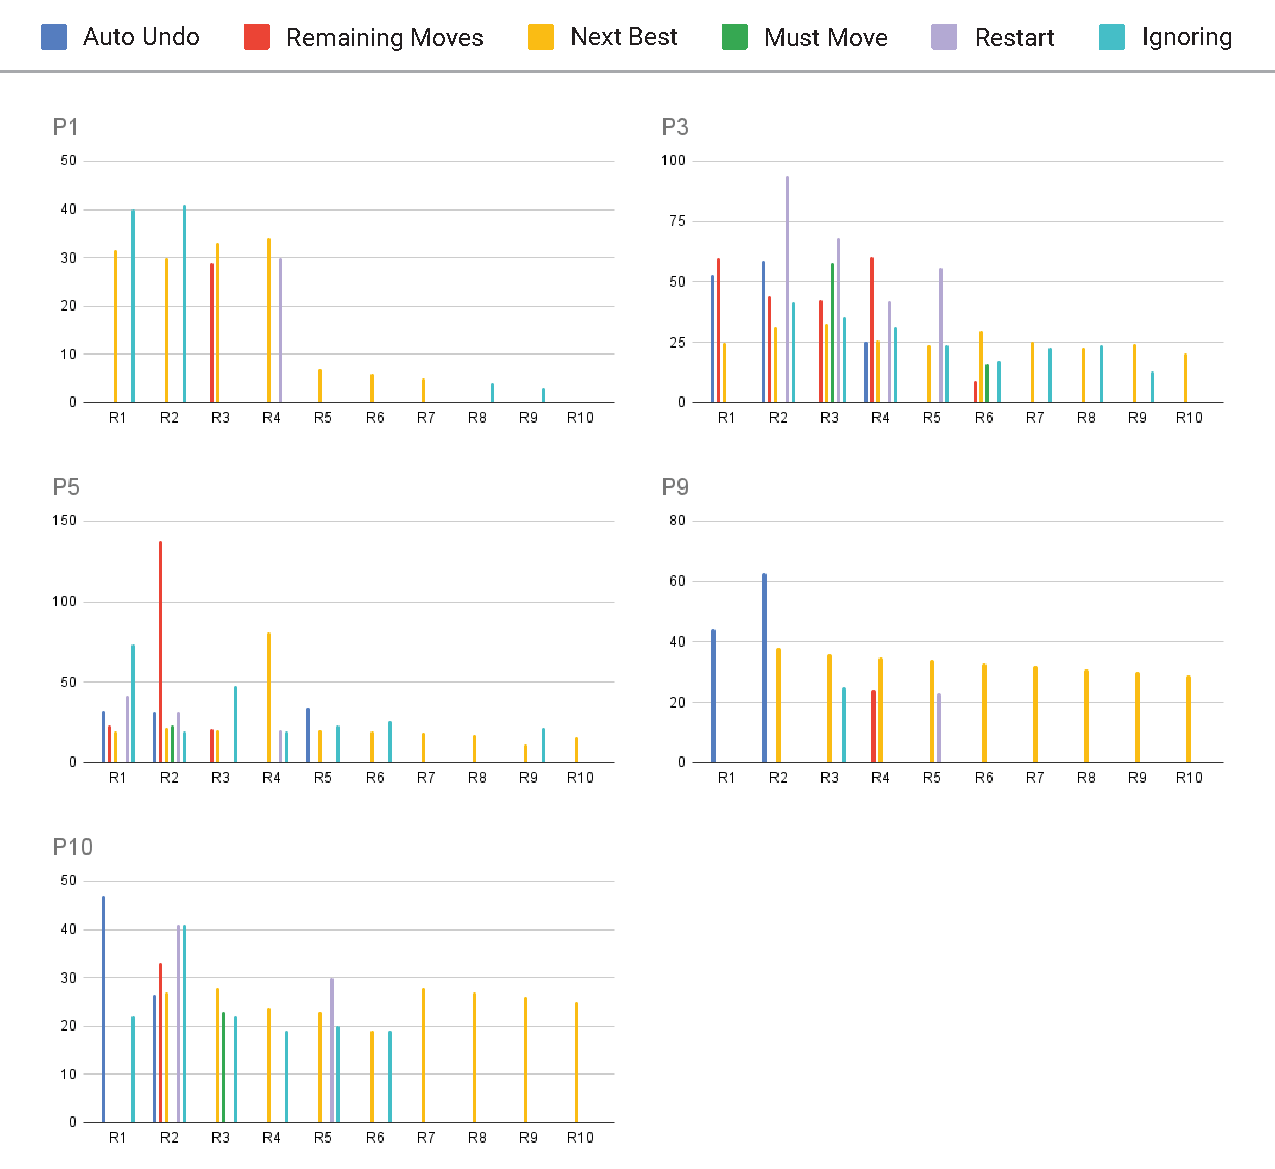
\includegraphics[width=\columnwidth]{img/set-3d.pdf}
  \caption{Hint request distribution for type E planning tasks}
  \label{fig:requesttypee}
\end{figure}

Figure~\ref{fig:requesttypem} illustrates how users request hints in type M planning tasks.
Table~\ref{tab:requesttypem} in the Appendix~\ref{apx:hintsstudy} contains the data used to generate the graphs in Figure~\ref{fig:requesttypem}.
Similar to type C and E, the hint ``Show the next best move'' is requested often in type M planning tasks.
For the planning task P7, the hint ``Show the remaining number of moves is requested more often compared to the other planning tasks in type M.
The ``Restart'' hint is not a common choice among subjects who attempted type M puzzles.
Only users attempting P13 planning task requested a restart.
The users attempting P13 planning task also moved the forbidden vehicle multiple times.
For the planning task P12, we only have one subject using the hints.
The subject requested the hint ``Show the vehicles that must be moved'' early in the planning task.
Then the user requested the ``Show the next best move'' hint 3 times and closer toward the end of the task opted to turn off the hints.

\begin{figure}[tpb]
  \centering
\includegraphics[width=\columnwidth]{img/requesttypem.png}
  \caption{Hint request distribution for type M planning tasks}
  \label{fig:requesttypem}
\end{figure}

\subsection{The Effectiveness of the Interactive Human-aware Intervention}
In Section~\ref{sec:relationshipavoidingforbidden}, we conclude that in order help the user avoid the forbidden vehicle, the Interactive Human-aware Intervention agent must direct the user toward the cost optimal solution for the planning task.
In this section, we evaluate how successful the interactive Human-aware Intervention model has been in moving the user's solution closer to the cost optimal solution using the hints.
Recall that the hints are properties derived from the cost optimal solution and the fact landmarks of $P_{observer}$.
We want to address the following questions:
\begin{enumerate}
\item Does the Interactive Human-aware Intervention have an effect on the solution length?
\item Does the Interactive Human-aware Intervention help move the user closer to the optimal solution?
\item Does seeing a help video affect the solution length?
\end{enumerate}

We introduce the following evaluation metrics.
\begin{enumerate}
\item The number of moves in the human user's solution
\item The difference from the cost optimal solution
\item The latest time a fact landmark is eventually achieved (landmark achievement)
\item The number of times a fact landmark is lost and regained (landmark regain)
\end{enumerate}
The definitions for these metrics will be presented later.
Question 1 is answered using the evaluation metric 1.
Question 2 is answered using the evaluation metrics 2, 3 and 4.
Question 3 is answered using the evaluation metrics 1.

For questions 1 and 2, we use the data from the control and condition groups for the planning tasks P1, P2, P4, P6, P7, P8, P9 and P10 for the evaluation.
We remove the planning tasks P3 and P5 because for those two tasks, the cost optimal solution while moving the forbidden vehicle is shorter than the cost optimal solution without moving the forbidden vehicle.
We also remove the planning tasks P11, P12 and P13 because these tasks are only used in the condition group.
For question 3 we use the data from the condition group and include the planning tasks P1 through P13.

\subsubsection{Using the Landmarks}
\label{sec:usingthelandmarks}
To derive the landmark based evaluation metrics, we examine how landmarks are achieved in cost optimal solutions generated by an automated planner for a given Rush Hour planning task.
We use the algorithm advanced by Hoffmann et al. \citeyear{hoffman2004lm} to generate the \textit{Greedy Necessary Fact Landmarks} for the planning task $P_{observer}$ and the actions that have the landmarks as post-conditions.
The algorithm uses a data structure called the Landmark Generation Graph (LGG) to find the landmarks and the greedy necessary orders between them. 
Nodes in LGG are the fact landmarks and the edges are the greedy necessary orders. 
Starting from the goal (the first landmark candidates), the algorithm uses the back-chaining process to find the earliest actions that can be used to achieve each landmark. 
Here, early means a greedy approximation of reachability from the initial state. 
The landmark achievers are actions grounded with the objects that must be moved to solve the planning task from the current state.

In order to analyze how the landmarks are achieved in the solution, we use the Fast Downward planner configured with the admissible heuristic Landmark-cut (\texttt{lmcut}) to generate 100 cost optimal plans for each planning task.
Figure~\ref{fig:achievement} illustrates how landmarks are achieved in five cost optimal plans for the planning tasks P1, P2, P4, P6, P7, P8, P9 and P10.
\begin{figure}[tpb]
  \centering
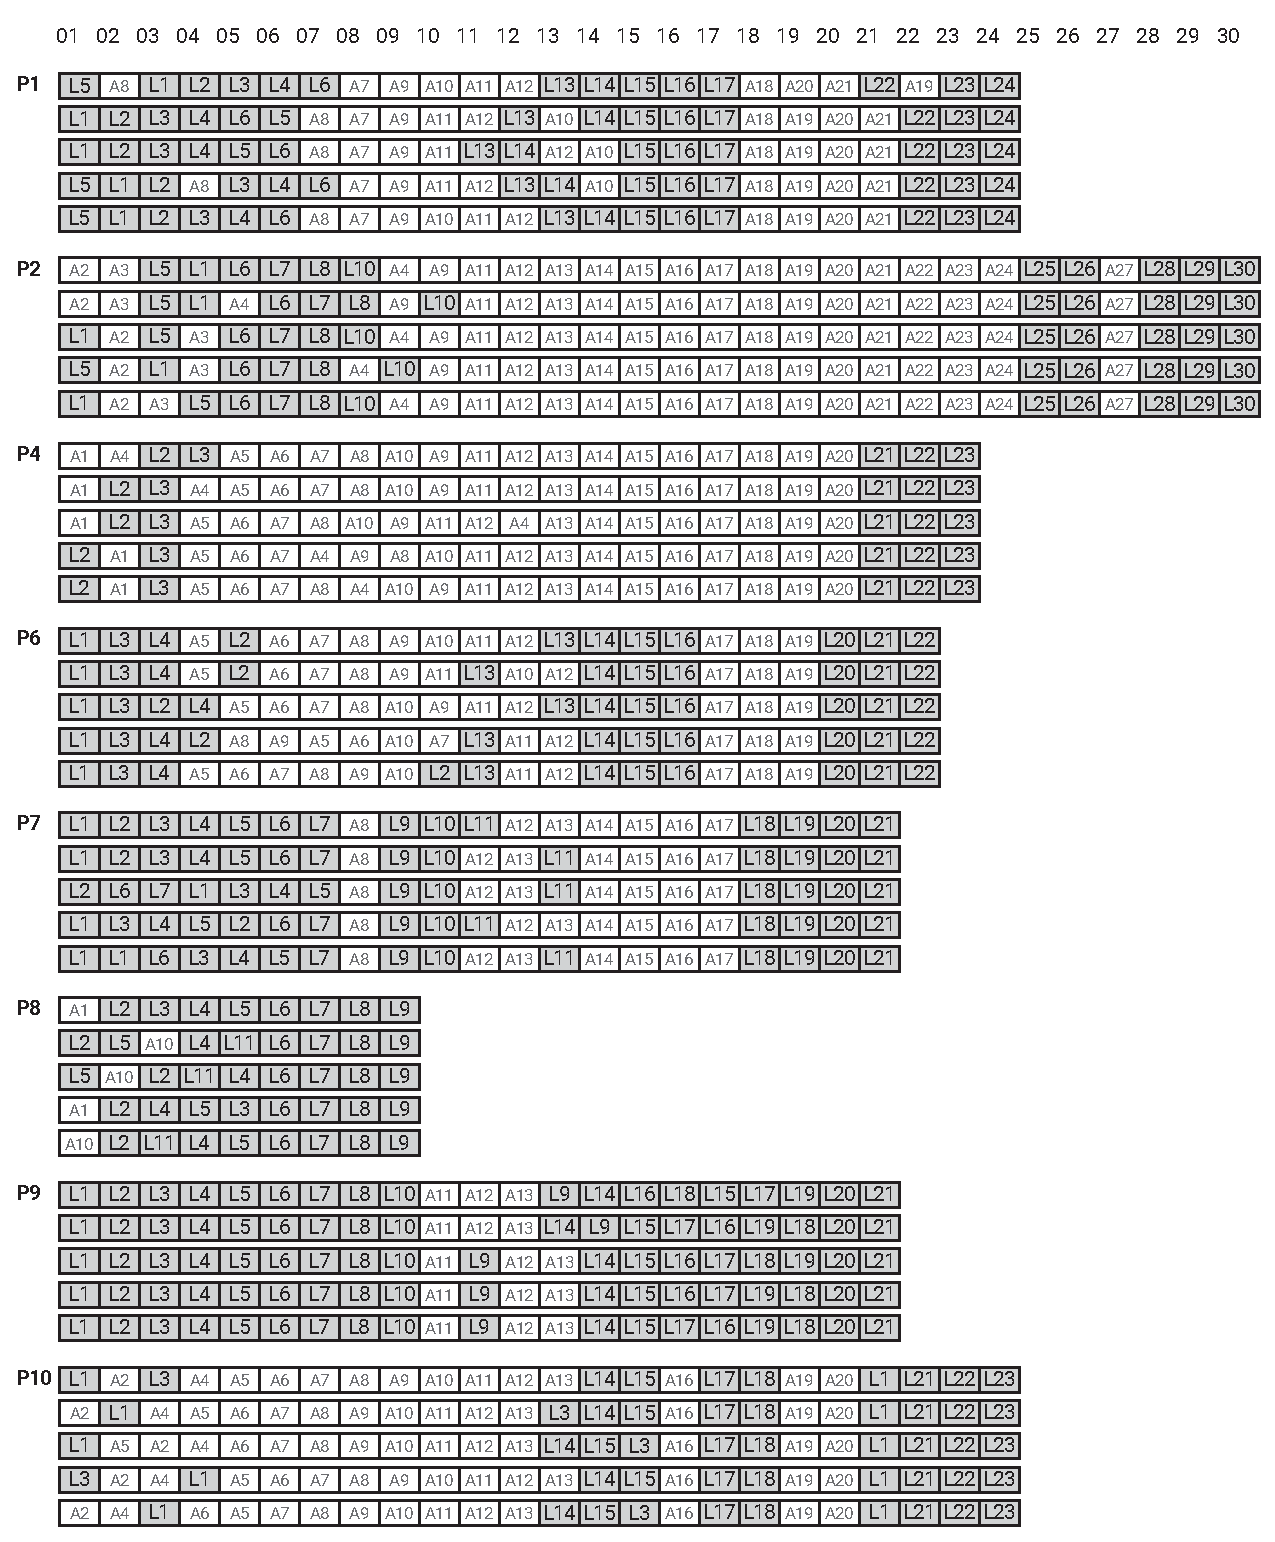
\includegraphics[width=\columnwidth]{img/landmarks.pdf}
  \caption{Landmark achieving patterns in five cost optimal solutions generated by the automated planner. The figures are scaled to reflect the solution length. Actions that achieve the landmarks are in gray cells. Other actions are in white cells. Note that the landmark identifiers L1, L2, $\ldots$ are unique to the planning task.}
  \label{fig:achievement}
\end{figure}
We manually examine the 100 cost optimal plans for each planning task identify frequently occurring landmark achievement patterns.
We see that in all cost optimal solutions the landmarks are achieved in \textit{clusters}.
We use the notation $[ Lj, \ldots ]$ to represent a \textbf{landmark cluster}, where $Lj, j\in\mathbb{N}$ refers to the landmark identifier.
Actions that are not landmarks that appear in the cost optimal plan are denoted with the identifier $(Ak, \ldots), k\in\mathbb{N}$.
Actions that the users execute, but do not appear in the cost optimal plans are denoted with the identifier $(Ul, \ldots), l\in\mathbb{N}$.
The landmark and action identifiers are unique to the planning task.
We denote this as $\langle Pi\rangle [Lj, \ldots] (Ak, \ldots) $, where $Pi$ refers to the planning task identifier, $i=\lbrace 1, 2, 4, 6, 7, 8, 9, 10\rbrace$.

There are groups of actions that achieve some landmarks early in the solution.
For example, consider the cost optimal solutions for the planning task P1 in Figure~\ref{fig:achievement}.
The cost optimal solution for P1 has 24 moves.
The cluster $[L1, L2, L3, L4, L5, L6]$ in the planning task P1 appear very early in the cost optimal solution.
The cluster $[L22, L23, L24]$ appear at the end most of the time.
The cluster $[L15, L16, L17]$ appear together in the middle after $L14$ has been achieved.
The cluster $[L13, L14]$ appear together in the middle before  the cluster $[L15, L16, L17]$.
The condensed representation applied to the cost optimal plans for the planning tasks P1, P2, P4, P6, P7, P8, P9, P10 are as follows:
\begin{itemize}
\item $\langle P1\rangle [L1, L2, L3, L4, L5, L6] (A8) (A7,A9) (A12) [L13, L14] (A10)$ \\ $[L15, L16, L17] (A18, A19, A20, A21) [L22, L23, L24]$
\item  $\langle P2\rangle [L1, L5, L6, L7, L8, L10] (A2, A3, A4, A9)$ \\ $(A11, A12, A13, A14, A15, A16, A17, A18, A19, A20, A21, A22, A23, A24)$ \\ $[L25 L26](A27)[L28, L29, L30]$
\item  $\langle P4\rangle [L2, L3](A1, A4, A5, A6, A7, A8, A9, A10, A11, A12, A13, A14, A15, A16, A17, A18, A19, A20)$\\$[L21, L22, L23]$
\item  $\langle P6\rangle [L1, L2,L3,L4](A5, A6, A7, A8, A9, A10)$ \\ $(A11,A12) [L13][L14, L15, L16](A17,A18,A19)[L20, L21, L22]$
\item  $\langle P7\rangle [L1, L2,L3,L4,L5,L6,L7,L9,L10](A8)[L11]$ \\ $(A12, A13, A14, A15, A16, A17)[L18,L19,L20,L21]$
\item  $\langle P8\rangle (A1,A10) [L2,L3,L4,L5,L6,L7,L8,L9,L10]$
\item  $\langle P9\rangle [L1,L2,L3,L4,L5,L6,L7,L8,L9,L10](A11, A12, A13)$\\$[L14,L15,L16,L17,L18,L19,L20,L21]$
\item  $\langle P10\rangle [L1,L3] (A2,A4,A5) (A6,A7,A8,A9,A10,A11,A12,A13) [L13,L14,L15](A16)$ \\ $[L17,L18] (A19,A20) [L1,L21,L22,L23]$
\end{itemize}

\begin{figure}[tpb]
\centering
	\begin{minipage}[b]{0.46\columnwidth}
	\includegraphics[width=\columnwidth]{img/landmarkp1.png}
	\caption{Human users achieving landmarks for the planning task P1}			
	\label{fig:p1}
	\end{minipage}
	\quad
	\begin{minipage}[b]{0.50\columnwidth}
	\includegraphics[width=\columnwidth]{img/landmarkp2.png}
	\caption{Human users achieving landmarks for the planning task P2}
	\label{fig:p2}
	\end{minipage}
\end{figure}

Although we can extract common patterns in achieving landmarks when the planning task is solved by an automated planner, this is not the case when human users solve planning tasks.
Figure~\ref{fig:p1} illustrates how two human subjects: A and B achieve the landmarks for the planning task P1 compared to an automated planner.
User B has achieved the landmarks for P1 similar to the automated planner.
There are also a few instances where the same landmark was lost and regained later (i.e. same y-value for different x-values).
Because user B achieved the landmarks similar to the automated planner, the user has been able to solve the planning task in fewer number of moves compared to the user A.
In contrast, user A has taken more number of moves to achieve the landmarks.
Consequently, user A's solution is longer.
Both user A and B has eventually achieved the landmark clusters similar to the automated planner.
Figure~\ref{fig:p2} illustrates how human subjects C and D achieve the landmarks for the planning task P2.
Here too, we can see how the landmark clusters are distributed within the solution produced by the automated planner.
We can see that user C has achieved the early landmark cluster similar to the automated planner.
However, some actions the user executed have caused him/her to lose those landmarks and having to regain them later around the $50^{th}$ move.
User D has lost the early landmark cluster twice before eventually regaining them around the $60^{th}$ move.
User C's solution is shorter compared to user D.
Therefore, when evaluating the human user solutions we monitor only the planning task's landmarks for when they are achieved for the last time and also how often they are regained.

We modify the condensed plan representation discussed above to include the two landmark evaluation metrics: (1) the latest time a fact landmark is eventually achieved and (2) the number of times a fact landmark is lost and regained.
We remove the actions that are not landmarks that appear in the cost optimal plan, i.e., $(Ak, \ldots), k\in\mathbb{N}$ as well as the actions that the users execute, but do not appear in the cost optimal plans, i.e., $(Ul, \ldots), l\in\mathbb{N}$.
The landmark cluster notation is modified as $[Lj(n), \ldots]$, where $Lj, j\in\mathbb{N}$ refers to the landmark identifier and $n\in\mathbb{N}$ corresponds to the evaluation metric value.
For example, if we use the new condensed plan representation for user A's solution to denote the latest time the landmarks are achieved, it will be as follows:
\begin{multline}
\langle P1\rangle [L1(6), L2(32), L3(33), L4(34), L5(1), L6(38)] [L13(37), L14(39)] \\ [L15(41), L16(42), L17(43)] [L22(49), L23(50), L24(51)]
\end{multline}
Using the new condensed plan representation for user A's solution to denote the number of times the landmarks are lost and regained:
\begin{multline}
\langle P1\rangle [L1(1), L2(2), L3(2), L4(2), L5(1), L6(2)] [L13(2), L14(2)] \\ [L15(1), L16(1), L17(1)] [L22(2), L23(2), L24(1)]
\end{multline}
The latest times when the landmarks are achieved by the human subjects attempting the planning tasks P1, P2, P4, P6, P7, P8, P9 and P10 with the Interactive Human-aware Intervention are shown in Tables~\ref{tab:p1landmarkachievement}, ~\ref{tab:p2landmarkachievement}, ~\ref{tab:p4landmarkachievement}, ~\ref{tab:p6landmarkachievement}, ~\ref{tab:p7landmarkachievement}, ~\ref{tab:p8landmarkachievement}, ~\ref{tab:p9landmarkachievement}, and ~\ref{tab:p10landmarkachievement} respectively.
The number of times a landmark is lost and regained for the planning tasks are shown in Tables~\ref{tab:p1landmarkregain}, ~\ref{tab:p2landmarkregain}, ~\ref{tab:p4landmarkregain}, ~\ref{tab:p6landmarkregain}, ~\ref{tab:p7landmarkregain}, ~\ref{tab:p8landmarkregain}, ~\ref{tab:p9landmarkregain}, and ~\ref{tab:p10landmarkregain}.

\subsubsection{Data Preparation for Evaluation Question 1}
We use the R statistical software for our analysis.
The control group has 113 observations.
The condition group has 68 observations.
Figure~\ref{fig:fullhisto} illustrates the frequency probability distribution of the number of moves in the solutions produced by the human users in the control and the condition groups. 
The data is highly skewed with a skewness factor +3.4.
\begin{figure}[tpb]
  \centering
\includegraphics[width=0.7\columnwidth]{img/histo_length.png}
  \caption{Frequency probability distribution of the number of moves}
  \label{fig:fullhisto}
\end{figure}

We remove 15 data points from the sample (8\%) to reduce the skewness and approximate the distribution of the number of moves to a normal distribution.
This adjustment resulted in 166 observations for the control and the condition groups.
The skewness factor of the adjusted sample is +0.89.
Given the skewness factor and also the sample size 166, greater than the recommended size by the Central Limit Theorem, we assume that this is a normal distribution.
Figure~\ref{fig:b1} shows the box plot for the distribution of the number of moves before the reduction of observations.
Figure~\ref{fig:b2} shows the box plot for the same after the reduction.
We use the adjusted sample for the statistical analyses that follow.

\begin{figure}[tpb]
\centering
	\begin{minipage}[b]{0.46\columnwidth}
	\includegraphics[width=\columnwidth]{img/outliers.png}
	\caption{Distribution of the number of moves before removing the outliers}			
	\label{fig:b1}
	\end{minipage}
	\quad
	\begin{minipage}[b]{0.50\columnwidth}
	\includegraphics[width=\columnwidth]{img/outliers_fixed.png}
	\caption{Distribution of the number of moves after removing the outliers}
	\label{fig:b2}
	\end{minipage}
\end{figure}

\subsubsection{Effect on the Number of Moves}
We address the question ``\textit{Does using the Interactive Human-aware Intervention (i.e., the hints) have an effect on the number of moves''}?
We propose the following study design.
\begin{itemize}
\item \textbf{Dependent variable}: Number of  moves
\item \textbf{Independent variables:}
\begin{itemize}
\item Used the Interactive Human-aware Intervention (Yes / No)
\item Planning Task Id (P1, P2, P4, P6, P7, P8, P9, P10)
\item Planning Task Type (C, E, M)
\end{itemize}
\end{itemize}

\noindent In Figure~\ref{fig:lenbypid}, the blue box plots represent the human subjects who used the Interactive Human-aware Intervention, while the red box plots represent the human subjects who did not.
We see that the median number of moves for planning tasks such as P1, P2, P4, and P6, the human subjects who used the Interactive Human-aware Intervention is higher.
On the other hand, the median number of moves is lower for the human subjects who solved the planning tasks P10, P7, and P9 using Interactive Human-aware Intervention.
For the planning task P8, the medians are almost the same between those who used the Interactive Human-aware Intervention and those who did not.
\begin{figure}[tpb]
  \centering
\includegraphics[width=0.9\columnwidth]{img/lenbypid.png}
  \caption{Box plot for the number of moves in the condition and the control group for each planning task}
  \label{fig:lenbypid}
\end{figure}

Figure~\ref{fig:lenbytype} shows the effect on the number of moves with the number of moves and planning task type (C, E, M) as factors.
Here too, the blue box plots represent the human subjects who used the Interactive Human-aware Intervention, while the red box plots represent the human subjects who did not.
Using the Interactive Human-aware Intervention, human subjects who solved type M planning tasks have been able to reduce the median number of moves.
In contrast, when using the Interactive Human-aware Intervention on type E and C puzzles the median number of moves have increased.

\begin{figure}[tpb]
  \centering
\includegraphics[width=0.7\columnwidth]{img/lenbytype.png}
  \caption{Box plot for the number of moves in the condition and the control group for each planning task type}
  \label{fig:lenbytype}
\end{figure}

We verify whether or not the observed differences in the number of moves between the control and the condition group are statistically significant.
Let $\mu_N$ be the mean number of moves in a solution from the control group (did not the Interactive Human-aware Intervention) and $\mu_H$ be the mean number of moves in a solution from the condition group (used the Interactive Human-aware Intervention).
Then, we define the null ($H_0$) and the alternative ($H_A$) hypotheses as follows.
\begin{itemize}
\item $H_0: \mu_N = \mu_H$, the means of the control and the condition group are the same.
\item $H_A: \mu_N \neq \mu_H$, the means of the control and the condition group are different.
\end{itemize}
Throughout, we use two-way ANOVA with the type \RomanNumeralCaps{3} correction to account for the unbalanced group design with $\alpha=0.05$.

When considering the planning task id and the usage of the Interactive Human-aware Intervention as factors, the effect of the planning task id on the number of moves is significant ($F<<<0, df=7$).
However, the effect of the usage of the Interactive Human-aware Intervention is not significant ($F=0.52, df=1$).
The interaction effect of the usage of the Human-aware Intervention and the planning task id is also not significant ($F=0.31, df=7$).
However, the Levene's Test to test the homogeneity of variance fails ($F=0.0007, df=15$) when considering the planning task id and the usage of the Human-aware Intervention as factors.
The homogeneity of variance is a critical requirement for the ANOVA test.
As it fails for this design, we ignore the results and do not draw any conclusions from the analysis.

In contrast, considering the planning task type and the usage of the Interactive Human-aware Intervention as factors, the Levene's Test to test the homogeneity of variance passes ($F=0.43, df=5)$.
Therefore, we report the conclusions from this design.
The effect of the planning task type on the number of moves is significant ($F<<<0, df=2$).
However, the effect of the usage of the Interactive Human-aware Intervention is not significant ($F=0.18, df=1$).
The interaction effect of the usage of the Human-aware Intervention and the planning task type on the number of moves is also not significant ($F=0.07, df=2$) at $\alpha=0.05$.
However, this interaction effect becomes significant at $\alpha=0.1$.
Therefore, at $\alpha=0.05$ we do not reject $H_0$ with respect to the usage of Interactive Human-aware Intervention and its effect on the number of moves.


\subsubsection{Effect on the Difference from the Number of Moves in the Cost Optimal Solution}
We address the question ``\textit{Does using the Interactive Human-aware Intervention (i.e., the hints) have an effect on the difference from the optimal''}?
This metric indicates how close the human user's solution has got to the cost optimal solution for the planning task in terms of the number of moves.
We propose the following study design.
\begin{itemize}
\item \textbf{Dependent variable}: 
\begin{multline}
\textup{Difference from the optimal} = \textup{Number of  moves in the user's solution}\\ - \textup{Number of moves in the cost optimal solution}
\end{multline}
\item \textbf{Independent variables:}
\begin{itemize}
\item Used the Interactive Human-aware Intervention (Yes / No)
\item Planning Task Id (P1, P2, P4, P6, P7, P8, P9, P10)
\item Planning Task Type (C, E, M)
\end{itemize}
\end{itemize}

In Figure~\ref{fig:lenoptbypid}, the blue box plots represent the human subjects who used the Interactive Human-aware Intervention, while the red box plots represent the human subjects who did not.
Similar to the case where the number of moves was the dependent variable, the median is higher for the human subjects who used the Interactive Human-aware Intervention for the planning tasks P1, P2, P4, and P6.
The human subjects who solved the planning tasks P10, P7, and P9 with the Interactive Human-aware Intervention resulted in a lower median.
For the planning task P8, there seems to be no difference between the medians of two groups.
\begin{figure}[tpb]
  \centering
\includegraphics[width=0.9\columnwidth]{img/lenoptbypid.png}
  \caption{Box plot for the difference from the optimal in the condition and the control group for each planning task id}
  \label{fig:lenoptbypid}
\end{figure}

Figure~\ref{fig:lenoptbytype} shows the effect on the  dependent variable by planning task type (C, E, M).
Using the Interactive Human-aware Intervention, human subjects who solved type M planning tasks have been able to reduce the median difference to the optimal.
In contrast, when using the Interactive Human-aware Intervention on type E and C planning task, the median differences to the optimal have increased.

\begin{figure}[tpb]
  \centering
\includegraphics[width=0.7\columnwidth]{img/lenoptbytype.png}
  \caption{Box plot for the difference from the optimal in the condition and the control group for each planning task type}
  \label{fig:lenoptbytype}
\end{figure}

We verify whether or not the observations for dependent variable between the control and the condition group are statistically significant.
Let $\mu_N$ be the mean difference to the optimal in a solution from the control group (did not the Interactive Human-aware Intervention) and $\mu_H$ be the mean difference to the optimal in a solution from the condition group (used the Interactive Human-aware Intervention).
Then, we define the null ($H_0$) and the alternative ($H_A$) hypotheses as follows.
\begin{itemize}
\item $H_0: \mu_N = \mu_H$, the means of the control and the condition group are the same.
\item $H_A: \mu_N \neq \mu_H$, the means of the control and the condition group are different.
\end{itemize}
Throughout, we use two-way ANOVA with the type \RomanNumeralCaps{3} correction to account for the unbalanced group design with $\alpha=0.05$.

As in the case where the dependent variable is the number of moves, the Levene's Test to test the homogeneity of variance fails ($F=0.0007, df=15$) for the design where we consider the planning task id and the usage of the Interactive Human-aware Intervention as factors.
Therefore, we ignore the results and do not draw any conclusions from the ANOVA.

In contrast, considering the planning task type and the usage of the Interactive Human-aware Intervention as factors, the Levene's Test to test the homogeneity of variance passes ($F=0.41, df=5)$.
Therefore, we report the conclusions from this design.
The effect of the planning task type on the differences to the optimal is significant ($F=0.001, df=2$).
However, the effect of the usage of the Interactive Human-aware Intervention on the differences to the optimal is not significant ($F=0.98, df=1$).
The interaction effect of the usage of the Human-aware Intervention and the planning task type on the differences to the optimal is also not significant ($F=0.01, df=2$) at $\alpha=0.05$.
However, this interaction effect becomes significant at $\alpha=0.1$.
Therefore, at $\alpha=0.05$ we do not reject $H_0$ with respect to the usage of Interactive Human-aware Intervention and its effect on the differences to the optimal.



\subsubsection{Computing the Evaluation Metric and the Data Preparation for Evaluation Question 2}
We use Figure~\ref{fig:latest} as an example to compute the evaluation metric, the latest time the landmarks are achieved.
In Figure~\ref{fig:latest}, there are three plans for the same planning task produced by an automated planner, user X and user Y respectively.
The plans are drawn in proportion to the number of steps.
The plan produced by the automated planner has 10 steps.
User X has produced a 20 step plan.
User Y has produced 25 step plan.
Let us assume L1, L2 and L3 are the landmarks for the planning task.
\begin{figure}[tpb]
  \centering
\includegraphics[width=\columnwidth]{img/latest.png}
  \caption{Plans produced by an automated planner (top), User X (middle) and User Y (bottom) achieving the same three landmarks.}
  \label{fig:latest}
\end{figure}
Table~\ref{tab:latest} shows the latest time in number of steps each landmark is achieved.
Note that User Y has initially achieved the L1 at step 8 but has lost and regained it at step 10.
Therefore the latest landmark achievement time for L1 for User Y is 10.
We compute the landmark achievement metric as follows:
\begin{equation}
\textup{landmark achievement} = \frac{\sum_{Li \in Landmarks} \left | (Li \textup{ latest achivement for user} - Li  \textup{ latest achievement for planner}) \right |}{|Landmarks|} 
\end{equation}
For the example in Figure~\ref{fig:latest}:
\begin{itemize}
\item landmark achievement for User X $= |(11-3)| + |(13-7)| + |(17-8)| = 23/3 \approx 8 steps$
\item landmark achievement for user Y $=|(10-3)| + |(16-7)| + |(22-8)|=30/3 = 10 steps$
\end{itemize}
Note that we compute the landmark achievement averaged over the number of landmarks in the planning task.
This is because different planning tasks used in this study have different number of landmarks.
In Section~\ref{sec:usingthelandmarks} we saw that the human users who achieve the landmarks for a planning task similar to the automated planner, find the solution to the planning task faster compared to human users who do not.
The landmark achievement metric captures this intuition.
The closer the user's solution is to the solution of the planner, the smaller the sum of the differences of achievement will be.
Thus, the metric indicates whether the user is getting closer to the optimal solution to the planning task or not.
Therefore, we use the landmark achievement metric to evaluate whether the Interactive Human-aware Intervention is helpful in moving the human user closer to the optimal solution produced by a planner.

\begin{table}[tpb]
\centering
\resizebox{0.25\textwidth}{!}{%
\begin{tabular}{|l|l|l|l|}
\hline
\multicolumn{1}{|c|}{\multirow{2}{*}{Plan}} & \multicolumn{3}{c|}{Landmark} \\ \cline{2-4} 
\multicolumn{1}{|c|}{} & L1 & L2 & L3 \\ \hline
Planner & 3 & 7 & 8 \\ \hline
User X & 11 & 13 & 17 \\ \hline
User Y & 10 & 16 & 22 \\ \hline
\end{tabular}%
}
\caption{Latest Landmark Achievement Times}
\label{tab:latest}
\end{table}

The control group has 113 observations.
The condition group has 68 observations.
Figure~\ref{fig:histach} illustrates the frequency probability distribution of the landmark achievement in the solutions produced by the human users in the control and the condition groups. 
The data is highly skewed with a skewness factor +4.2.
\begin{figure}[tpb]
  \centering
\includegraphics[width=0.7\columnwidth]{img/histo_ach.png}
  \caption{Frequency probability distribution of the landmark achievement}
  \label{fig:histach}
\end{figure}

We remove 24 data points from the sample (13\%) to reduce the skewness and approximate the distribution of the landmark achievement to a normal distribution.
This adjustment resulted in 159 observations for the control and the condition groups.
The skewness factor of the adjusted sample is +0.95.
Given the skewness factor and also the sample size 159, greater than the recommended size by the Central Limit Theorem, we assume that this is a normal distribution.
Figure~\ref{fig:b3} shows the box plot for the distribution of the landmark achievement before the reduction of observations.
Figure~\ref{fig:b4} shows the box plot for the same after the reduction.
We use the adjusted sample for the statistical analyses that follow.

\begin{figure}[tpb]
\centering
	\begin{minipage}[b]{0.46\columnwidth}
	\includegraphics[width=\columnwidth]{img/outliers_ach1.png}
	\caption{Distribution of the landmark achievement before removing the outliers}			
	\label{fig:b3}
	\end{minipage}
	\quad
	\begin{minipage}[b]{0.50\columnwidth}
	\includegraphics[width=\columnwidth]{img/outliers_ach2.png}
	\caption{Distribution of the landmark achievement after removing the outliers}
	\label{fig:b4}
	\end{minipage}
\end{figure}

\subsubsection{Effect on the Latest Time the Landmarks Are Achieved}
We address the question ``Does using the Interactive Human-aware Intervention have an effect on the landmark achievement?''
We propose the following study design.
\begin{itemize}
\item \textbf{Dependent variable}: landmark achievement
\item \textbf{Independent variables:}
\begin{itemize}
\item Used the Interactive Human-aware Intervention (Yes / No)
\item Planning Task Id (P1, P2, P4, P6, P7, P8, P9, P10)
\item Planning Task Type (C, E, M)
\end{itemize}
\end{itemize}

In Figure~\ref{fig:achbypid}, the blue box plots represent the human subjects using the Interactive Human-aware Intervention, while the red box plots represent the human subjects who do not.
The median landmark achievement for the human subjects using the Interactive Human-aware Intervention for the planning tasks P1, P2, P4, and P6 is higher.
The median landmark achievement for P10 when using Interactive Human-aware Intervention is slightly higher.
The human subjects who solved the planning tasks P7, and P9 with the Interactive Human-aware Intervention reported lower median landmark achievement.
For the planning task P8, there is a slight reduction in the median landmark achievement when using Interactive Human-aware Intervention.
\begin{figure}[tpb]
  \centering
\includegraphics[width=0.9\columnwidth]{img/achbypid.png}
  \caption{Box plot for the landmark achievement in the condition and the control group for each planning task id}
  \label{fig:achbypid}
\end{figure}

Figure~\ref{fig:achbytype} shows the effect on the dependent variable by planning task type (C, E, M).
Using the Interactive Human-aware Intervention, human subjects who solved type M planning tasks have been able to reduce the median landmark achievement.
In contrast, when using the Interactive Human-aware Intervention on type E and C planning task, the median landmark achievement have increased.
\begin{figure}[tpb]
  \centering
\includegraphics[width=0.7\columnwidth]{img/achbytype.png}
  \caption{Box plot for the landmark achievement in the condition and the control group for each planning task type}
  \label{fig:achbytype}
\end{figure}

We verify whether or not the observations for dependent variable between the control and the condition group are statistically significant.
Let $\mu_N$ be the mean landmark achievement in a solution from the control group (did not the Interactive Human-aware Intervention) and $\mu_H$ be the mean landmark achievement in a solution from the condition group (used the Interactive Human-aware Intervention).
Then, we define the null ($H_0$) and the alternative ($H_A$) hypotheses as follows.
\begin{itemize}
\item $H_0: \mu_N = \mu_H$, the means of the control and the condition group are the same.
\item $H_A: \mu_N \neq \mu_H$, the means of the control and the condition group are different.
\end{itemize}
Throughout, we use two-way ANOVA with the type \RomanNumeralCaps{3} correction to account for the unbalanced group design with $\alpha=0.05$.

When using Interactive Human-aware Intervention and the planning task id as factors to the dependent variable landmark achievement, the Levene's Test to test the homogeneity of variance fails ($F=0.0001, df=15$) for the design.
Therefore, we ignore the results and do not draw any conclusions from the ANOVA.

In contrast, considering the planning task type and the usage of the Interactive Human-aware Intervention as factors, the Levene's Test to test the homogeneity of variance passes ($F=0.14, df=5)$.
Therefore, we report the conclusions from this design.
The effect of the planning task type on the landmark achievement is significant ($F=0.003, df=2$).
The effect of the usage of the Interactive Human-aware Intervention on the landmark achievement is also significant ($F=0.04, df=1$) at $\alpha=0.05$.
The interaction effect of the usage of the Human-aware Intervention and the planning task type on the landmark achievement is not significant ($F=0.64, df=2$).
Therefore, at $\alpha=0.05$ we reject $H_0$ with respect to landmark achievement considering the usage of Interactive Human-aware Intervention and the planning task type.
We conduct TukeyHSD post-hoc analysis to identify whether the landmark achievement difference changes significantly based on whether the subject use Interactive Human-aware Intervention or not (i.e. the combinations, Y:C-N:C, Y:M-N:M and Y:E-N:E). 
The result show that the differences in the mean landmark achievement is not significant for any of the three categories.


\subsubsection{Computing the Evaluation Metric and the Data Preparation for Evaluation Question 2}
We use the example illustrated in Figure~\ref{fig:latest} to compute the evaluation metric, the number of times the landmarks are regained.
In the example, the planner has achieved each landmark L1, L2, L3 only once.
User X has also achieved each landmark only once.
User Y has achieved the landmark L1 twice: initially achieved the at step 8 but has lost and regained it at step 10.
Therefore, Y has regained the landmark once.
Additionally Y has achieved the landmarks L2 and L3 only once.
We compute the landmark regain metric as follows:
\begin{equation}
\textup{landmark regain} = \sum_{Li \in Landmarks} \left | (\textup{number of times } Li \textup{ appears in the solution} - 1) \right |
\end{equation}
For the example in Figure~\ref{fig:latest}:
\begin{itemize}
\item landmark regain for User X $= |(1-1)| + |(1-1)| + |(1-1)| = 0$
\item landmark regain for user Y $=|(2-1)| + |(1-1)| + |(1-1)| = 1$
\end{itemize}
In Section~\ref{sec:usingthelandmarks} we saw that the human users who achieve the landmarks for a planning task similar to the automated planner, find the solution to the planning task faster compared to human users who do not.
The landmark achievement metric captures this intuition.
Furthermore, for the Rush Hour planning tasks the cost optimal solutions achieve each landmark only once in most cases.
When the user gains a landmark and loses it by executing another action, it indicates that the user is getting away from the solution.
The closer the user's solution is to the solution of the planner, the smaller the landmark regain value will be.
Thus, the metric indicates whether the user is getting closer to the optimal solution to the planning task or not.
Therefore, we use the landmark regain metric to evaluate whether the Interactive Human-aware Intervention is helpful in moving the human user closer to the optimal solution.


The control group has 113 observations.
The condition group has 68 observations.
Figure~\ref{fig:histreg} illustrates the frequency probability distribution of the landmark achievement in the solutions produced by the human users in the control and the condition groups. 
The data is highly skewed with a skewness factor +3.5.
\begin{figure}[tpb]
  \centering
\includegraphics[width=0.7\columnwidth]{img/histo_regain.png}
  \caption{Frequency probability distribution of the landmark regain}
  \label{fig:histreg}
\end{figure}

We remove 18 data points from the sample (10\%) to reduce the skewness and approximate the distribution of the landmark achievement to a normal distribution.
This adjustment resulted in 163 observations for the control and the condition groups.
The skewness factor of the adjusted sample is +1.3
There are many zeros in the data set, indicating that many subjects achieved the landmarks only once.
Given the sample size 163 being greater than the recommended size by the Central Limit Theorem, we assume that this is a normal distribution.
Figure~\ref{fig:b5} shows the box plot for the distribution of the landmark achievement before the reduction of observations.
Figure~\ref{fig:b6} shows the box plot for the same after the reduction.
We use the adjusted sample for the statistical analyses that follow.

\begin{figure}[tpb]
\centering
	\begin{minipage}[b]{0.46\columnwidth}
	\includegraphics[width=\columnwidth]{img/outliers_regain.png}
	\caption{Distribution of the landmark regain before removing the outliers}			
	\label{fig:b5}
	\end{minipage}
	\quad
	\begin{minipage}[b]{0.50\columnwidth}
	\includegraphics[width=\columnwidth]{img/outliers_regain_fixed.png}
	\caption{Distribution of the landmark regain after removing the outliers}
	\label{fig:b6}
	\end{minipage}
\end{figure}


\subsubsection{Effect on Regaining Landmarks}
We address the question ``Does using the Interactive Human-aware Intervention have an effect on the landmark regain?''
We propose the following study design.
\begin{itemize}
\item \textbf{Dependent variable}: landmark regain
\item \textbf{Independent variables:}
\begin{itemize}
\item Used the Interactive Human-aware Intervention (Yes / No)
\item Planning Task Id (P1, P2, P4, P6, P7, P8, P9, P10)
\item Planning Task Type (C, E, M)
\end{itemize}
\end{itemize}

In Figure~\ref{fig:regainbypid}, the blue box plots represent the human subjects using the Interactive Human-aware Intervention, while the red box plots represent the human subjects who do not.
The median landmark regain for the human subjects using the Interactive Human-aware Intervention for the planning tasks P1, P4, and P6 is higher.
The median landmark regain for the human subjects using the Human-aware Intervention for the planning tasks P2, P7 and P9 is lower.
The medians for P8 and P10 are almost the same.

\begin{figure}[tpb]
  \centering
\includegraphics[width=0.9\columnwidth]{img/regainbypid.png}
  \caption{Box plot for the landmark regain in the condition and the control group for each planning task id}
  \label{fig:regainbypid}
\end{figure}

Figure~\ref{fig:regainbytype} shows the effect on the dependent variable by planning task type (C, E, M).
Using the Interactive Human-aware Intervention, human subjects who solved type M planning tasks have been able to reduce the median landmark regain.
In contrast, when using the Interactive Human-aware Intervention on type E and C planning task, the median landmark regain have increased.
\begin{figure}[tpb]
  \centering
\includegraphics[width=0.7\columnwidth]{img/regainbytype.png}
  \caption{Box plot for the landmark regain in the condition and the control group for each planning task type}
  \label{fig:regainbytype}
\end{figure}

We verify whether or not the observations for dependent variable between the control and the condition group are statistically significant.
Let $\mu_N$ be the mean landmark regain in a solution from the control group (did not the Interactive Human-aware Intervention) and $\mu_H$ be the mean landmark regain in a solution from the condition group (used the Interactive Human-aware Intervention).
Then, we define the null ($H_0$) and the alternative ($H_A$) hypotheses as follows.
\begin{itemize}
\item $H_0: \mu_N = \mu_H$, the means of the control and the condition group are the same.
\item $H_A: \mu_N \neq \mu_H$, the means of the control and the condition group are different.
\end{itemize}
Throughout, we use two-way ANOVA with the type \RomanNumeralCaps{3} correction to account for the unbalanced group design with $\alpha=0.05$.

When using Interactive Human-aware Intervention and the planning task id as factors to the dependent variable landmark achievement, the Levene's Test to test the homogeneity of variance fails ($F<<<0, df=15$) for the design.
The  Levene's test also fails for the design that considers the Interactive Human-aware Intervention and the planning task type ($F=0.04, df=5$).
Therefore, we ignore the results and do not draw any conclusions from the ANOVA.

\subsubsection{Effect of Help Video}
We address the question ``Does seeing a help video move the user closer to the optimal solution?''.
For the analysis we use the data from the Interactive Human-aware Intervention  human subject study, where 135 participants completed 13 planning tasks.
Recall that during the experiment the participants were randomly assigned to two groups where one group watched a 44 second help video on how to solve the Rush Hour planning task while avoiding the forbidden vehicle.
The other group did not watch the help video.
72 subjects watched the help video, while 63 subjects did not.
We propose the following study design.
\begin{itemize}
\item \textbf{Dependent variable}: Number of moves
\item \textbf{Independent variables:}
\begin{itemize}
\item Used the Interactive Human-aware Intervention (Yes / No)
\item Watched the help video (Yes/No)
\item Planning Task Id (P1 through P13)
\item Planning Task Type (C, E, M)
\end{itemize}
\end{itemize}
We join the two variables: using the Interactive Human-aware Intervention and watching the help video to form one independent variable with 4 levels.
Level 1, Yes-Yes indicates that the participant used both kinds of help.
Level 2, Yes-No indicates that the participant used the Interactive Human-aware Intervention but did not watch the video.
Level 3, No-Yes indicates that the participant did not use the Interactive Human-aware Intervention but watched the help video.
Level 4, No-No indicates that the participant did not use either kind of help.
We use this combined variable for our analysis.
There are 55 users in level 1, 16 in level 2, 52 in level 3 and 12 in level 4.

Figure~\ref{fig:histvid} illustrates the frequency probability distribution of the number of moves for the solutions produced by the human users in the sample. 
The data is highly skewed with a skewness factor +4.6.
\begin{figure}[tpb]
  \centering
\includegraphics[width=0.7\columnwidth]{img/histo_video.png}
  \caption{Frequency probability distribution of the number of moves}
  \label{fig:histvid}
\end{figure}
We remove 8 data points from the sample (5\%) to reduce the skewness and approximate the distribution of the number of moves to a normal distribution.
This adjustment resulted in 127 observations for the sample.
The skewness factor of the adjusted sample is +0.67.
Given the skewness factor and also the sample size 127, greater than the recommended size by the Central Limit Theorem, we assume that this is a normal distribution.
Figure~\ref{fig:b7} shows the box plot for the distribution of the number of moves before the reduction of observations.
Figure~\ref{fig:b8} shows the box plot for the same after the reduction.
We use the adjusted sample for the statistical analyses that follow.

\begin{figure}[tpb]
\centering
	\begin{minipage}[b]{0.46\columnwidth}
	\includegraphics[width=\columnwidth]{img/outliers_vid.png}
	\caption{Distribution of the number of moves before removing the outliers}			
	\label{fig:b7}
	\end{minipage}
	\quad
	\begin{minipage}[b]{0.50\columnwidth}
	\includegraphics[width=\columnwidth]{img/outliers_fixed_vid.png}
	\caption{Distribution of the number of moves after removing the outliers}
	\label{fig:b8}
	\end{minipage}
\end{figure}

In Figure~\ref{fig:helpsbypid}, the box plots represent the human subjects using the four levels of help for the 13 planning tasks.
The frequency distribution in the sample for the planning tasks and each category of help type is shown in Table~\ref{tab:help}.
\begin{table}[tpb]
\centering
\resizebox{0.3\textwidth}{!}{%
\begin{tabular}{|l|c|c|c|c|}
\hline
\multicolumn{1}{|c|}{\multirow{2}{*}{\begin{tabular}[c]{@{}c@{}}Planning\\ Task\end{tabular}}} & \multicolumn{4}{l|}{Help Category} \\ \cline{2-5} 
\multicolumn{1}{|c|}{} & \multicolumn{1}{l|}{YY} & \multicolumn{1}{l|}{YN} & \multicolumn{1}{l|}{NY} & \multicolumn{1}{l|}{NN} \\ \hline
P1 & 1 & - & 5 & - \\ \hline
P2 & 4 & - & 4 & - \\ \hline
P3 & - & 8 & - & 5 \\ \hline
P4 & 8 & - & 6 & - \\ \hline
P5 & - & 8 & - & 7 \\ \hline
P6 & 5 & - & 5 & - \\ \hline
P7 & 6 & - & 1 & - \\ \hline
P8 & 6 & - & 3 & - \\ \hline
P9 & 4 & - & 5 & - \\ \hline
P10 & 3 & - & 5 & - \\ \hline
P11 & 6 & - & 7 & - \\ \hline
P12 & 5 & - & 5 & - \\ \hline
P13 & 8 & - & 6 & - \\ \hline
\end{tabular}%
}
\caption{Frequency distribution in the sample for the planning task id and the types of help}
\label{tab:help}
\end{table}

\begin{figure}[tpb]
  \centering
\includegraphics[width=\columnwidth]{img/helpsbypid.png}
  \caption{Box plot for the number of moves in the sample for the planning task id and the types of help they received}
  \label{fig:helpsbypid}
\end{figure}

\begin{figure}[tpb]
  \centering
\includegraphics[width=0.7\columnwidth]{img/helpsbytype.png}
  \caption{Box plot for the number of moves in the sample for each planning task type and the type of help they received}
  \label{fig:helpsbytype}
\end{figure}
Figure~\ref{fig:helpsbytype} shows the effect on the dependent variable by planning task type (C, E, M).
We verify whether or not the observations for dependent variable between the control and the condition group are statistically significant.
We define the null ($H_0$) and the alternative ($H_A$) hypotheses as follows:
\begin{itemize}
\item $H_0$: there is no difference in the mean number of moves for any help type.
\item $H_A:$, there is a difference in the mean number of moves for help types.
\end{itemize}
We use two-way ANOVA with $\alpha=0.05$.

When using the help type and the planning task type as factors to the dependent variable number of moves, the Levene's Test to test the homogeneity of variance fails ($F=0.02, df=7$) for the design.
Therefore, we ignore the results and do not draw any conclusions from the ANOVA.
The  Levene's test passes for the design that considers the help type and the planning task id ($F=0.29, df=25$).
We report the ANOVA results for this design, which shows that the there is a significant difference in the mean number of moves when considering the four levels of help types ($F=0.001, df=3$).
Thus we reject $H_0$.
The mean number of moves is also significant when considering each planning task ($F<<<0, df=11$).
However, the mean number of moves difference considering the help type and the planning task interaction is not significant ($F=0.49, df=2$).

Since the planning task type significantly affects the number of moves in a solution, we want to find out for individual planning tasks whether or not using the help type has an effect on the number of moves.
For example, is the difference in mean number of moves for YY and NY for planning task P1 significant?, is the difference in mean for YY and NY for planning task P2 significant? and so on.
We conduct the TukeyHSD posthoc analysis to compare the pair-wise means.
For the planning tasks P1 the mean number of steps used by YY category is lower than the NY category. However, this difference is not statistically significant.
For the planning task P2, the mean number of steps used by YY category is higher than the NY category. However, this difference is not statistically significant.
For the planning task P3, the mean number of steps used by YN category is higher than the NN category. However, this difference is not statistically significant.
For the planning task P4, the mean number of steps used by YY category is higher than the NY category. However, this difference is not statistically significant.
For the planning task P5, the mean number of steps used by YN category is higher than the NN category. However, this difference is not statistically significant.
For the planning task P6, the mean number of steps used by YY category is lower than the NY category. However, this difference is not statistically significant.
For the planning task P7, the mean number of steps used by YY category is higher than the NY category. However, this difference is not statistically significant.
For the planning task P8, the mean number of steps used by YY category is lower than the NY category. However, this difference is not statistically significant.
For the planning task P9, the mean number of steps used by YY category is higher than the NY category. However, this difference is not statistically significant.
For the planning task P10, the mean number of steps used by YY category is slightly lower than the NY category. However, this difference is not statistically significant.
For the planning task P11, the mean number of steps used by YY category is higher than the NY category. However, this difference is not statistically significant.
For the planning task P12, the mean number of steps used by YY category is higher than the NY category. However, this difference is not statistically significant.
For the planning task P13, the mean number of steps used by YY category is higher than the NY category. However, this difference is not statistically significant.


\section{Discussion}
We introduce four properties of the solution to the observer's planning problem $P_{observer}$ as hints: \textbf{the number of remaining moves}, \textbf{the next best move}, \textbf{the vehicles that must be moved} and \textbf{restart planning task}.
The subjective preference ratings the human subjects gave for the helpfulness of the hints agree with the frequency the users requested the hint.
For all there planning task types (C, E, M), the human subjects rated the ``\textbf{Show the next best move}'' as the highest in helpfulness.
When considering the actual use of hints the hint ``Show the next best move'' hint was the most frequently requested hint for all three planning task types (C, E, M).
This finding indicates that when human users are stuck during the Rush Hour planning task (i.e., getting close to moving the forbidden vehicle) they subjectively prefer information that tells directly them what to do next.
In contrast, the ``Number of remaining moves'' and the ``Vehicles that must be moved'' are \textit{heuristic information} of the planning problem $P_{observer}$.
The heuristic information forces the human user to think deeply about the planning task instead of giving direct instructions.
Our experiments show that the human users do not respond well to heuristic related information about the Rush Hour planning problem when they are offered as help.

We introduce four metrics to evaluate whether or not the Interactive Human-aware Intervention has been successful in helping the user find the solution to the planning task, while avoiding the forbidden vehicle as follows:
\begin{itemize}
\item The number of moves in the human user's solution
\item The difference from the cost optimal solution
\item The landmark achievement
\item The landmark regain
\end{itemize}
Although the 13 planning tasks we selected for this study produce optimal solutions having approximately the same number of moves (except for P8), the experiments show that the human users have difficulty getting closer to the optimal solution even with the use of hints.
The longer the human users spend exploring the search space of the planning task, the higher the likelihood that he/she will also move the forbidden vehicle.
When examining the cost optimal plans produced by an automated planner, we see that the landmarks are typically achieved in clusters.
However, when examining the solutions produced by the human users, we see that they lose and regain the landmarks several times before eventually achieving them.
The closer the human user's solution resembles the solution produced by the automated planner in terms of when the landmark clusters are achieved, the closer the number of moves will be to that of the optimal solution for that planning task.
Therefore, information intended to guide the human user toward the solution to the Rush Hour planning task must be designed to help the user achieve the landmarks quicker.
Furthermore, the guiding information needs to be presented to the user as direct instructions.

Let us now revisit the questions we intended to answer through our evaluation.
\begin{enumerate}
\item Does the Interactive Human-aware Intervention have an effect on the solution length?
\item Does the Interactive Human-aware Intervention help move the user closer to the optimal solution?
\item Does seeing a help video affect the solution length?
\end{enumerate}
When we resolve question 1 using the number of moves as the evaluation metric, we find that for some planning tasks the Interactive Human-aware Intervention pushes the user closer to the optimal solution. However, the effect is not statistically significant considering the $\alpha=0.05$ for the study sample.
When we resolve question 2 using the difference from the cost optimal solution, the landmark achievement and the landmark regain as evaluation metrics, we find that the differences from the cost optimal solution and the landmark achievement between those who used Interactive Human-aware Intervention and those who did not are not statistically significant.
The distribution of landmark regain for the sample violated the homogeneity  of variances assumption for ANOVA. 
Therefore, we do not report the results for that metric to answer question 2.
We also find that metrics number of moves, difference to the optimal and landmark achievement change significantly considering planning task ids.
The change is also statistically significant.
When we resolve question 3 using the number of moves as the evaluation metric, we find that there is a statistically significant difference between the types of help used (video and hints) between the 13 planning tasks.
However, because each planning task is different from one another (even within the same category C, E, M) we want to find out if the number of moves differ significantly for the subjects attempting the same planning task, while using different help types.
Posthoc analysis did not reveal a significant difference in the number of moves for the pair-wise comparisons for this question.
I think reducing the number of planning tasks to one each from the categories C, E, M will help us yeild more conclusive results on the effects of the Interactive Human-aware Intervention.


For the experiment, we categorized the Rush Hour planning tasks into three types by the position of the forbidden vehicle.
However, when examining the solutions produced by the human users there are large variances in the number of moves within the planning tasks that fall into one category.
For example, consider the planning task P2 and P8 in the same category where the forbidden car is placed in the corner of the board.
The minimum number of moves in a plan produced by a human user for task P2 is 67 and the maximum number of moves is 419.
For task P8 the minimum number of moves is 9 and the maximum number of moves is 14.
This allows us to draw the conclusion that there are yet undiscovered factors  about the Rush Hour planning task, besides the position of the forbidden vehicle, which contribute to the difficulty the human users experience in finding the solution.
Some example factors that may determine the difficulty may be how blocked the forbidden vehicle is on the board, the number of vehicles blocking the path of the goal car.
It is also likely that the difficulty may be determined by a combination of these factors.

We set a threshold for the number of steps for the Human-aware Intervention to start making predictions. 
The threshold is required to generate enough data for the classifier to predict intervention and minimize the false alarms early on in the planning task, which may cause the user to turn off the alerts.
However, it was observed that many human users moved the forbidden vehicle within the window in which predictions were absent.
This indicates that the human users need guidance early on in the planning task.
It may be helpful to design intervention prediction models to reduce the size of this window.
